%----------------------------------------------------------------------------------------
%	PACKAGES AND OTHER DOCUMENT CONFIGURATIONS
%----------------------------------------------------------------------------------------

\documentclass[12pt]{report} 
% Default font size is 12pt, it can be changed here

\usepackage[none]{hyphenat}

\usepackage{geometry} % Required to change the page size to A4
\geometry{a4paper} % Set the page size to be A4 as opposed to the default US Letter

\usepackage{graphicx} % Required for including pictures

\usepackage{listings}

\usepackage{cleveref}

\crefname{subsection}{subsection}{subsections}

\usepackage{tikz}

\usepackage{float} % Allows putting an [H] in \begin{figure} to specify the exact location of the figure
\usepackage{wrapfig} % Allows in-line images such as the example fish picture

\usepackage{lipsum} % Used for inserting dummy 'Lorem ipsum' text into the template

\linespread{1.2} % Line spacing

%\setlength\parindent{0pt} % Uncomment to remove all indentation from paragraphs

\graphicspath{{Pictures/}} % Specifies the directory where pictures are stored

\setlength\parindent{0pt}

\begin{document}

%----------------------------------------------------------------------------------------
%	TITLE PAGE
%----------------------------------------------------------------------------------------

\begin{titlepage}

\newcommand{\HRule}{\rule{\linewidth}{0.5mm}} % Defines a new command for the horizontal lines, change thickness here

\center % Center everything on the page

\textsc{\LARGE Vrije Universiteit Brussel}\\[1.5cm] 
\textsc{\Large Operating Systems and Security}\\[0.5cm] 
\textsc{\large Mini-project essay}\\[0.5cm] 

\HRule \\[0.4cm]
{ \huge \bfseries High availability and scalability on GNU/Linux clusters}\\[0.4cm] % Title of your document
\HRule \\[1.5cm]

\begin{minipage}{0.4\textwidth}
\begin{flushleft} \large
\emph{Author:}\\
Pieter Libin % Your name
\end{flushleft}
\end{minipage}
~
\begin{minipage}{0.4\textwidth}
\begin{flushright} \large
\emph{Professor:} \\
Prof. Dr. Timmerman\\
\emph{Assistant:} \\
Mr. Fayyad-Kazan
% Supervisor's Name
\end{flushright}
\end{minipage}\\[4cm]

{\large \today}\\[3cm] % Date, change the \today to a set date if you want to be precise

%\includegraphics{Logo}\\[1cm] % Include a department/university logo - this will require the graphicx package

\vfill % Fill the rest of the page with whitespace

\end{titlepage}

%----------------------------------------------------------------------------------------
%	TABLE OF CONTENTS
%----------------------------------------------------------------------------------------

\tableofcontents % Include a table of contents

\newpage % Begins the essay on a new page instead of on the same page
         % as the table of contents 

\chapter*{Preface}
\section{Source code}
When I reference to source code files, this will always be in the src
directory. This directory can be found in this public github.com
project: https://github.com/plibin-vub/OSSEC-mini-project.
\section{Videos}
For some demonstrations I created a video, I've put these videos on
Youtube and reference to them in this document via their YouTube URL.
\section{Naming conventions}
Server names are always expressed using single quotes (e.g.: 'node1').
\section{Presentation}
Before the presentation, I will hand in the following deliverables:
\begin{itemize}
\item this final report
\item the final presentation
\item a directory with all the edited videos
\item a directory with all pictures that I used in the report
\item source code (the src directory on github)
\item the base ubuntu virtual machine, which I used to derive all
  other virtual machines from (root-password=''empty'', root-user=''plibin'')
\end{itemize}
During the presentation, I will present some videos that depict
experiments that I executed (most of the videos in the deliverable).

\chapter{Introduction} % Major section
\section{Abstract}
Nowadays, several web-applications exist (Facebook, Wikipedia, Twitter, ...) that serve millions of users concurrently. To achieve this, huge clusters are in place, where each cluster node serves a large amount of users. In order to assure the availability of such applications, it is required that whenever a cluster node crashes, the systems remains responsive and handles subsequent requests by another cluster node.\\
The number of users of such web applications can vary greatly over different time intervals (e.g.: Twitter tends to be under heavy load upon the arrival of significant events). Also, when an application gains in popularity, the number of users grows quickly in a short timespan. This requires an application to be able to scale in the number of users it can serve.\\
This project situates these concepts in the general ICT landscape and makes a detailed analysis on the importance of availability and scalability provisions on GNU/Linux server clusters.\\
The project identifies a set of technologies that are available on the GNU/Linux platform to set up a system that can assure high availability and support proper scalability for both computational and storage nodes. The selected technologies will be tested in a simulated cluster setting.\\
In the last phase of the project, a high-availability and scalable
cluster simulation is constructed that mimics the functionality of
Wikipedia.

\section{Interest}
A big amount of today's software applications runs on remote servers, and
this amount will most likely grow even more in the near future. In
order to allow users to have a good experience, it is vital that the
application remains available at all times. For applications that only are
used by a handful of users, this might be an easy task by just
providing a redundant server, however, for applications that are used
by thousands (or millions) of concurrent users, this task becomes
quite complex.\\
Another aspect is that such applications need to be able to scale; a
sudden rise in popularity may cause an application to be used by a
x-fold of users from one day to another.\\
These considerations of high-availability and scalability interest me
greatly because they have a huge impact how application are
hosted; and this again determines how such applications are to be
implemented.\\
In my opinion, having an overview and understanding of the technologies and
architectures that high-availability and scalability setups use,
is a big asset for a computer scientist.\\
Next to this, I have always been fascinated by large data centers,
while the hardware of such setups is no longer my main interest (this
is more inclined to software these days) I still remain intrigued how
the different components in such setups interact.

\section{Relevance}
A lot of huge companies (Google, Facebook, Microsoft, ...) and
organisations (Wikipedia, ...) depend on available and scalable
application \footnote{And the number of companies that operate in the
  ``Cloud'' seems to grow every days}. This makes
high-available and scalability solutions economically relevant.
Also in the High Performance Computing domain high-available and
scalability solutions become more and more important to operate huge
research clusters. Such research clusters are essential for scientists
and companies to do research.

\chapter{General scope of high-availability and scalability}
This project will focus on GNU/Linux clusters, however,
the aspect of high-availability and scalability are not limited to
this domain. In this chapter, I present a short overview of the
importance of these aspects in other domains.

\section{Airplane/car/spacecraft software}
\subsection{On-board computers}
Cars and planes that are released today are operated by millions of lines of code
\cite{ieee_cars_and_planes}. It is of course vital in such devices
that there is a high level of availability; important systems (breaks,
steering, ...) should be available in a redundant way. \\
Another important aspect is that failure should be detected as soon as
possible; if certain parts of a car don't function any more (or only
partly) without the vehicle being aware of this, a very dangerous
situation can arise.\\
For spacecrafts, the same rules apply when considering passenger
safety. However, also unmanned flights, such as the mars exploration missions
need to consider an extra dimension of availability. These vehicles
can only be controlled by on-board computers or via a satellite
up-link (where signals take 1 to 1.5 hours \cite{mars_rover} to go
from one end to the other). These vehicles have a
huge development and production cost, which is an extra motivation to
 keep the system running as long as physically possible.
\subsection{Computer Aided Design}
The design of vehicles can be assisted with several software
solutions, these software packages require a lot of computational
power and can benefit from the use of High Performance Clusters
\cite{hpc_cars}.

\section{Healthcare}
\subsection{Patient monitoring}
For patient monitoring equipment, it is vital that these devices
report problems as soon as possible. Usually these devices can be
quickly replaced with a working unit, but now knowing that a device is
corrupted might cost patient lives.\\

\subsection{Drug development}
As a side node, I want to mention here for drug development both
academic researchers and pharmaceutical company staff use High
Performance Clusters intensively to study the effects of drugs
\cite{deforche2007bayesian} \cite{lengauer2006bioinformatics}.

\subsection{Desktop systems}
The stability of desktop computers has improved a lot of the last decade,
mainly by stabilising desktop operating systems. A huge source of system
crashes in the past were buggy device drivers that made the entire
operating system crash.
Current desktop operating systems
(e.g.: Windows NT) are built to recover from such crashes
\cite{windows_nt_kernel}.

\subsection{Home entertainment systems}
These appliances (TV's, game consoles, media center) are used by users via a limited interface (e.g.:
remote controls) and users expect them to work without any problems
(as their VCR a  couple of decades ago).\\
While system crashes still might accepted on the desktop, this is
definitely not the case on these kind of devices. 


\chapter{Different aspects in cluster availability}
\label{chap:aspects}
\section{Hardware}
\subsection{Servers}
Servers are the processing nodes in a cluster, they contain a CPU
(often more than one), memory (often a significant amount), one or
more network interfaces, a power supply (often 2 for redundancy) and
usually one or more hard disks.\\
Several server-cases exists:
\subsubsection{Tower server} 
A tower server is comparable to a desktop PC tower. It's cheap, but it is
  an inconvenient format to use in cluster rooms.
\subsection{Rack server}
These servers are build as thin boxes that can be stacked on top of each other in a rack.
\subsection{Blade server}
A blade server is a large computer that is able to contain multiple
  blades. A blade is essentially a slice containing memory, a CPU and a
  disk. The power and networking is managed by the surrounding case.
 Blade servers are convenient for cluster setups since they
   allow to replace (broken) blades very easily.
\subsection{Network}
The network infrastructure connects the different elements in the
cluster and allows the application
that runs on the cluster to connect to the internet.\\
Several components are used to setup cluster networks:
\begin{itemize}
\item switches
\item routers
\item firewalls
\end{itemize}
\subsection{Storage}
Storage can be integrated in a server. There 
also exists solutions that implement storage that can be directly
integrated in the network:
\begin{itemize}
\item network attached storage 
\item storage area network
\end{itemize}
There are also separate units that can be connected to a server
directly (with no network in between) : direct-attached storage.
\subsubsection{Disk types}
There currently exist two types of disks: hard disk drives (HDDs) and
solid state disks (SSDs). A HDD contains rotating platters and 
stores data by magnetising parts of the disk. An SSD is fully
implemented in an integrated electronic circuit; it contains no moving
parts at all (comparable to a USB flash drive).\\
Overall, SSDs (which are only ``recently'' on the market) have a much better
performance. However, traditional HDDs still offer a much better
price/MB ratio than SSDs do.\\
Therefore the choice of using HDDs or SSDs usually depends on the
problem you want to solve: quickly accessing a limited amount of data
vs storing vast amounts of data that are only issued
periodically \footnote{The two systems are often used in combination,
so the technologies can complement each other}.

\section{Infrastructure}
\subsection{Sites}
Big companies such as Google, Facebook, Microsoft, ... have there own
sites to host their clusters. Smaller companies often start by hosting
their applications at a third party's site. Some of this third party
providers offer servers that are can be completely administered by their
users (e.g.: rackspace \cite{rackspace}, Amazon EC2 \cite{amazon_ec2}), others provide cloud
platforms that allows the users to simply install an application
(e.g.: Google App Engine \cite{google_app_engine}).

\subsection{Location}
An important aspect to consider is the distance of
the cluster to the end users. When this distance is too big, users will suffer from the
network connection's latency. For example: between the US
and Europe, a latency of $\approx 90ms$ can be expected
\cite{verizon_latency}.
This is a significant number when we consider that a latency of 1/10th
of a second (100ms) already starts to feel slow for an end user 
\cite{web_app_latency}.\\
Therefore it is beneficial to have the data center as close to the end
user as possible.\\

Another important aspect is the climate of the region where the data
center is located. Data centers tend to get hot and cooling down the
datacenter can become an expensive (and carbon-unfriendly) issue.
A solution can be to move the datacenter to a colder region 
\cite{datacenter_cold}.\\

Proximity to an energy provider is another factor that needs to be
considered (see \cref{energy_provider}).

\subsection{Buildings}
The buildings that host a data center need to take a set of precautions to
avoid or handle natural disasters such as floods, fires, earthquakes
and extreme weather.\\
The buildings should be well secured (physically), since quite often, 
private data of end-users will reside on the servers in the
building.\\
Applying passive architectural techniques can allow
the data center to consume dramatically less power \cite{passive_architecture}.
 
\subsection{Energy providers}
\label{energy_provider}
Data centers might produce their own power on-site by
using solar panels on the top of the roofs or even building a dedicated
power plant.\\
It should be taken under consideration whether a country / region has
 trustworthy energy providers (which can be a problem in development 
countries).\\
A company will negotiate a contract that guarantees the availability of power
within a reasonable degree of certainty.\\
The datacenter should be able to handle short power-outs by using
UPSs. To deal with longer power-outs diesel-powered generators can be used.\\
Considering climate change, the cost of energy might rise
significantly over the next years, rendering these aspects even more important.

\section{Internet Availability}
Most companies will work with a third party provider to setup a
connection with the Internet. \\
A company will negotiate a contract that guarantees the availability of Internet
within a reasonable a reasonable degree of certainty.\\

\section{Storage}
A proper backup strategy should be in place. This strategy will depend
on the companies' resources and the importance of the different
datasources.
Some general guidelines for backups (based on \cite{ha_book}):
\subsubsection{Mirroring does not replace backups}
If a file
is removed by a human error, a mirrored solution will not be able to
restore the data.
Additionally, it is still possible that these disks will
fail at the same time
(for example when the power is interrupted).

\subsubsection{Backups are more often used to fix human errors
  than to fix a disaster}
For this reason, it is important that restoring data can happen
quickly.

\subsubsection{Regularly test the restore procedure}
It is always possible that there is a hardware problem or some backup
rule is invalidated. To make sure this is not discovered in the case
of a disaster, it is important to regularly test both the hardware and
the restore procedures.

\subsubsection{Handle hardware (and tapes) with care}
A lot of backups are made on tapes, such cartridges are particularly
sensitive to dust and moist, so it is important to store them
appropriately.

\subsubsection{Only use a tape as many times as the producer
  guarantees it will work}
Tapes have an expiration date, make sure to stop using them after this
date. If you dispose of them, make sure to destroy them thoroughly,
since they might contain private data.

\subsubsection{Multiple locations}
If you can afford it, it is always better to distribute backups over
multiple physical locations. In case there goes anything seriously
wrong in one of the data centers, it is still possible to recover from
this.

\section{Database systems}
The following two (mainly) database technologies are currently used in cluster
settings: Relational database management systems and NoSQL systems.

\subsection{Relational database management systems}
This technology is based on the relational model \cite{codd}. It
allows data to be modelled as tables that represent entities. These
entities are then connected using relations (basically pointers from
one table to another).\\
It is possible to query the information in the model using the
declarative language SQL.\\
RDBMs implement ACID
and transactions, two features which are very
useful for application developers, but make scaling RDBMs difficult.

\subsection{NoSQL databases}
The concept of NoSQL databases was introduced as a reaction on the
difficulties of scaling out RDBMs. While RDBMs store data using a relational
model, most NoSQL solutions simply act as a key-value store ($\approx$
a distributed dictionary data structure).\\
NoSQL databases are usually simpler in design and allow for easier horizontal
scaling \cite{wikipedia_nosql}.\\
However, since data is simply stored in a key-value store, joining
over multiple datasets (which can be easily done with RDBMs) has to be
implemented on top of the NoSQL database (doing this might still
be slow \cite{nosql_problems}). \\

\section{Application crashes}
Software will never be perfect, therefore there will always be a
chance that a program crashes. Important is that developers try to
create defensive software, that rather than to crash will show an
appropriate error message.\\
That said, since we cannot built a high-availability cluster assuming
our software will not crash, we need to try to contain the crashes as
good as possible.\\
When software is implemented as a process that runs in the user space,
it cannot crash the entire operating system, but only that specific process (if
there are no bugs in the operating system). In my opinion this is
essential to ensure the stability, if not, one error can ultimately
take down the entire cluster.\\
But still, if we have a web server that is written in C/C++, when an
error occurs in one of the applications threads, this can potentially
bring down the entire application server. Java applications can cope
better with these kind of errors: when one application thread throws
an exception the application server (Tomcat, JBoss, ...) can continue
to serve the other users.\\ 
In order to ensure that an error in a  C/C++ program does not crash the entire
application (and all sessions that are tied to it),  a process can be
assigned to each application session, however, running the application
like this will require more computational resources.\\
When one session of the application throws an error and the
application server can properly recover from it (by using one of the
techniques described in the previous paragraphs), we can show the
user an appropriate error message or try to continue this user's
session in another thread/process.\\
Another very important remark : when a crash happens, it is important
to properly log what is wrong and inform an administrator about this
problem. This way the problem can be investigated and hopefully
fixed. 
Because it is not always possible to look what is
going on on the production server, it is important for the logging to
be as complete as possible. This way developers and administrators can try to
reproduce the problem without the need to access the production system.

\section{Human error}
A lot of problems are introduced by human errors: bugs in
applications, bugs in operating systems, errors in architectures and
their implementation, ...\\
While it makes sense to have redundancy in hardware, it makes equally
sense to have redundancy in developers and system administrators.\\
For developers, it is vital to have peer reviews, or even pair
development techniques for the more complicated parts of a system.\\
System administrators often take decisions that can impact huge parts
of a cluster, so it would probably be a good idea to double-check such
decisions before actually applying them. This can be done by first
applying the changes on a test setup before pushing them to the
production cluster \footnote{Its vital for system administrators to
  have a sandbox that allows them to perform realistic tests}.\\
It is also important that the knowledge of systems and processes is
well distributed over employees, in case any of the employees leaves,
the system can still be operational. Therefore it is also important
that architectures, procedures and system layouts are thoroughly
documented, and that this documentation is kept up to date. 

\section{Operating systems}
GNU/Linux is very popular in cluster settings
\cite{server_market_share}.
The GNU/Linux operating system is known for its speed and stability.
It is however important to note that the kernel has a monolithic
design, while this makes it a fast kernel, it also allows system drivers
to crash the entire kernel (in extremis). \\
Since clusters will usually use reputed well-tested hardware that has
good driver support for the Linux kernel, this is usually not  a big
problem.\\
When an operating system does crash for some reason (a bug, or a
hardware failure) this should be dealt with appropriately, for example
by restarting the cluster node that has crashed or (if the crashed
node cannot be started again) by starting a new node that will take
the crashed node's place.\\
When a crash happens, it is essential to investigate what went wrong,
so lessons can be learned and actions can be takes to avoid the
problem from happening again.

\section{Monitoring}
It is important to monitor the status of a cluster, to take actions in
case there is something wrong. On the other hand, we should also take
care not to overload the network by constantly polling nodes.\\
Two aspects are particularly important when monitoring: 
\begin{itemize}
\item gathering usage statistics (CPU usage, network load, ...)
\item diagnose problems in time, and act on them
\end{itemize}

\section{Virtualization}
Virtualization is a technique that is used a lot in cluster
environments. It allows us to deal with server resources in a more
abstract fashion.\\
This allows certain actions to be automated in an easier way;
for example: restarting a node only requires invoking a program.\\
Furthermore, it allows server resources to be split up easier; one
virtualised node can use a part of the physical memory of an
underlying server, or only 1 of the set of CPUs the underlying server
has installed.\\
Virtualising hardware has some costs in terms of performance, however,
these days, several hardware provisions are in place to further
improve the performance of virtual machines (e.g.: Intel's Hardware-Assisted
Virtualization Technology \cite{intel_havt}, AMD Virtualization
\cite{amd_virt}).

\section{Different kinds of outages}
I will present an overview of the different kind of outages that are
possible (based on \cite{ha_book}):
\subsection{Hardware}
Hardware can fail whether it is new or old. Especially prone for
defect are the moving parts in a computer: the HDDs, tape drives,
tape libraries and fans.\\
To extend the computer's lifetime, the machine needs to be properly
cooled \footnote{A sufficient amount of fans is required and the room needs to
be air conditioned}. \\
There should be as little dust in the room as possible to avoid the
fans to get dirty (and eventually fail).\\
The life-time of servers that run constantly under heavy load is
considered to be 3 years \cite{ms_cloud_cost}.

\subsection{Environmental and physical failure}
\subsubsection{Natural disasters}
\begin{itemize}
\item earth quakes
\item fires
\item floods
\item extreme weather
\end{itemize}
\subsubsection{Infrastructure failure}
\begin{itemize}
\item cables that break
\item air conditioning that breaks down
\item UPSs or diesel generators that fail
\end{itemize}
\subsubsection{Third party delivery failure}
\begin{itemize}
\item internet delivery failures
\item power delivery failures
\end{itemize}

\subsection{Network failures}
It is possible that network components fail (this can be connected to
error in hardware and/or
software). Also problems with the DNS or DHCP servers might occur.\\
Distributed Denial-of-service (DDOS) or other security 
 attacks can also shutdown an entire network.

\subsection{Application failures}
All layers of an application can experience problems: the web/application
server, the database or the actual application. It is important to be
aware of this and write applications in a defensive way.

\section{Definition of high availability, expectations and realistic
  goals}
\subsection{Definition of high availability}
I use the definition used in \cite{ha_book}:\\
``Availability is a measure of the time that is server is functioning
normally''.\\
Availability can be calculated with this formula \cite{ha_book}:
$A=\frac{MTBF}{MTBF +
  MTTR}$ \footnote{MTBF = mean time between failures, MTTR = mean time to repair}.\\
An example: to achieve 99.9999 \% availability one is permitted to 6
minutes downtime in 11.4 years! This is highly improbable to be
achieved \cite{ha_book}.\\
A more realistic goal could be 10 minutes downtime per year, this is
expressed as an availability of 99.998\% \cite{ha_book}.

\subsubsection{Expectations and realistic goals}
Unavailability can cost lots of money: people of your online web shop
might leave and look for another shop, imageinge the stock market that is not
able to respond, ...\\
However, we should always try to be realistic in our expectations, if 50\%
of a company's data centers fail, there is a good chance not everyone
will still be able to be server, however, this is such a far-fetched
scenario that it is probably not cost-effective to try to preempt
it.\\
No matter how good an infrastructure is setup, there are always
aspects that are beyond our control \cite{black_swan}, so it is
important to be careful promising availability percentages to
customers. 

\chapter{Scalability and its effects on economy and environment}
\section{Power consumption}
The power consumed by large web applications is huge. As an
example, in 2011 Facebook consumed 532 million kilowatt hours of
energy and Google consumed 2 billion kilowatt hours of
energy in 2010 \cite{datacenter_power} \footnote{As a comparison:
  Belgium used 84 billion kilowatt hours in 2008}

\section{Software efficiency}
For some companies (such as Facebook) one of the reasons why this
power consumption is so high is that it takes a lot of computation to
render PHP pages \cite{facebook_php}. Facebook in particular is trying
to fix this by creating a PHP virtual machine \cite{php_vm}.\\
Note that using more efficient programming language such as Java or C++ 
from the start of such projects might make these kind of efforts
obsolete.

\section{Climate change}
Needless to say that numbers in the range of Google's or Facebook's
power usage contribute significantly to climate change. Since it can
be expected that the demand for cloud solutions will only go up, my
opinion is that green data centers \footnote{And applications!} will become more
important in the near future.\\

\chapter{Identifying high availability and scalability solutions}
\section{Cluster nodes}
\subsection{Cluster node monitoring}
The two major monitoring tools on GNU/Linux platforms are Nagios and
Ganglia. Both tools implement several monitoring aspects, but the
focus of each of the tools is different. Nagios is more oriented
towards detecting system problems and sending out notifications for
such events, while Ganglia provides a long term overview of the status
of cluster nodes. To ensure high availability, detecting problems is
the most important aspect. The sooner problems are revealed, the
sooner actions can be undertaken to avoid any impact on end users. It
is important that problems are properly communicated to system
administrators, since they might be able to further investigate the
problem. In the event of any hardware failure the intervention of
an administrator will be required. However, it is also necessary to
execute programs to repair the state of the cluster
 upon the detection of failure. Nagios specialises on both these
 issues \cite{nagios:2013}.
In order to make new nodes available when necessary, we need to
monitor the resource availability on all of the online nodes.
Monitoring statistics also allows system engineers to gain insight in
performance needs of an application over the course of time. 
Such statistics can also be used to setup models that can be used to
predict system load \cite{andreolini:2006}. Ganglia collects these
kind of statistics and stores them in a round-robin database, namely RDDTool
\cite{ganglia:2013} \cite{rrdt:2013}.

\section{Computational cluster nodes}
\subsection{Application monitoring}
Monitoring a cluster node is not enough to guarantee that it is
properly servicing clients. It is possible that the application (for
example: the web application server) has gotten in an infinite loop,
and as such is using practically all of the CPU's power, but in reality is
processing no new client request.
A possibility to monitor applications is to keep track of the number of
client request per seconds (or another appropriate time unit) that get
processed and compare it with the amount of computational resources
that is used.
This number of client requests is very application specific; a web
server might process thousands client requests per second, while a
server responsible for rendering a scene in an animated movie might only process
one request per hour \cite{apm:2013}.
This information usually can be extracted from the log files generated
by the server application (for example: the request log file for
Apache httpd). This information than can be pass to Ganglia to be
stored and monitored together with the other server's statistics
\cite{ganglia:2013}.

\subsection{Cluster node management}
In large cluster environments, it is not possible to wait for
a human intervention when a problem occurs. Therefore, when nodes or
applications fail, the monitor server should restart them.
There are several systems that allow for programs to restart
physical servers that reside in a rack (for example Dell's DRAC).
Since I will only use a simulated cluster in this mini-project, I will
only deal with starting and stopping virtualised nodes \footnote{Which I think should
be a valuable contribution taken into account the large amount of
virtualised server that are used in data centers these days}.
I will use VirtualBox to set up my simulated cluster, this
virtualization software has support to start and stop virtual machines
using the command line.
When an application stalls but the operating system is still fully
functioning, the monitoring server can decide to restart the server application, or
(if the application has support for this) simply kill the thread that
is responsible for the problems.

\subsection{Load balancing proxies}
\label{sec:load_balancing_proxies}
Load balancing is a method for distributing workloads across multiple
computing nodes. It can be used to improve the reliability of a system through
redundancy and to provide scalability by sending requests to the most
available node.
Load balancing has several applications such as High Performance
Clusters, database servers, and HTTP servers. In this section I will
focus on HTTP load balancing.
A prominent TCP/HTTP load balancing proxy is HAProxy.
\cite{haproxy:2013}. This software supports a set of
balancing algorithms \cite{tarreau:2006}, most notably:
\begin{itemize}
  \item round robin: each server is used in turns, taking into account
    the different server's weights (these weights can be configured
    per server and can be adjusted on the fly)
  \item balance leastconn: the server with the lowest number of connections receives the connection
  \item source/uri: this algorithm hashes respectively the source IP
    or URI of the request, this hash is than divided by the total
    weight of the running servers to determine which server should
    receive the request
\end{itemize}
HAProxy also supports Access Control Lists configurations that allow
the load balancer to select a server based on a header in the HTTP
request. When multiple server clusters exists in different countries
and/or continents, this feature allows us to connect a user to a
server that is located near his own location.
Another important aspect to consider when setting up a load balancing
infrastructure for HTTP servers is that many dynamic web applications
rely on session context \cite{tarreau:2006}. Since this session context is usually stored
on the web server, it is necessary for the load balancer to pass the
client's request to the same web server: this is called persistence.

\section{Storage and backup}

\subsection{Data replication}
Data replication implies that the same date is stored on multiple
data storage systems. This should be transparent to the end user: the
user should not be aware of this when using the data (note that when
working with a multi-tier architecture, it is possible that the
`end-user'  is represented by another tier in the system).
Data replication is relevant for both:
\begin{itemize}
\item high availability systems: to ensure a smooth transition from a
  failing data storage node to a working node
\item systems that require scalability: to make load balancing possible
\end{itemize}
We can distinguish 3 types of data replication
\cite{datareplication:2013} :

\subsubsection{Database replication}

\paragraph*{Master-slave replication}
In this setup, there exists one master database, this database is the only instance
that accepts updates. When an update statement is received by the
master database, it is applied to the database and appended to the log. The statements
in this log are than propagated to the slave databases.
Most database systems support this replication strategy (Postgres \cite{postgres_db:2013},
MySQL \cite{mysql_db:2013}, ...).

\paragraph*{Multi-master replication}
In this setup, multiple master instances exists, each of these master
instances accept updates. These updates are than communicated with the
other master instances. 
This has the advantages that :
\begin{itemize}
\item the master node can fail without interrupting the system
\item the update load can be distributed over multiple nodes
\end{itemize}
There are also some significant disadvantages related to this technique:
\begin{itemize} 
\item increased complexity
\item most implementations violate the ACID constraints
\item to fix conflicts that may arise between different database
  instances, resources of the database nodes are required and
  communication between the conflicted nodes will increase the network
  traffic
\end{itemize}
Note that there are other techniques to accommodate the advantage of
load balancing mentioned above: database shards, NoSQL (reference to
this section).

\subsubsection{Disk storage replication}
Disk storage replication collects updates to a block device and
applies these updates collectively to multiple devices.
This can be implemented in hardware, the functionality is than
embedded in the array disk controller.
DRBD \cite{drbd_soft:2013} implements this functionality in software.
This software allows users to mirror disks within a system or over a
network (the DRBD website explains this as follows: ``DRBD can be
understood as network based RAID-1'' \cite{drbd_soft:2013}).

\subsubsection{File-based replication}
Disk storage replication replicates entire block devices, however for
some applications, it might be necessary to only replicate parts of
the logical file system.
\paragraph*{Batch replication}
To replicate file systems in batch, synchronisation tools such as
rsync \cite{rsync_software:2013} can be
used. The rsync Unix tool can synchronise 2 directories from one location to the
other (this can be done over a network). The advantage compared to a
simple ``scp -r'' is that rsync will only transfer the changes by using
delta encoding.
\paragraph*{Real-time replication}
I was not able to find any tools on GNU/Linux that allow real-time
file-based replication based with default filesystems such as ext4.
It is however possible to achieve this kind of file-based replication
by using one of the distributed file systems, which I will discuss in
the next section.

\subsection{Backup}
In order to setup a reliable backup system, some technologies
are required: 
\begin{itemize}
\item the ability to take a snapshot of a file system: this can be
  achieved by using the Logical Volume Manager, which is part of the
  mainline Linux kernel \cite{linux_kernel_soft:2013}
\item the ability to take snapshots and incremental backups of RDBMs: most RDBMS systems
  support this; some examples:
  \begin{itemize}
  \item Postgres: via barman \cite{barman_software:2013}
  \item MySQL: via mysqldump (and by enabling the binary log)
  \end{itemize}
\item the ability to make incremental filesystem backups; this can be
  done using rsync \cite{rsync_software:2013}
\end{itemize}

\subsection{Distributed file systems}
\label{ceph}
Distributed file systems share storage using a network protocol, they
deliver scalability and failure
correction in such a way that it is transparent to the client.
Such filesystems can restrict access to certain files based on access lists
and/or file system quotas. Distributed file systems allow clients to
access files in the same way as they would be able to do on their
local file system \footnote{A client might refer to an end user, 
but it might as well refer to one of the tiers in a multi-tier
system}.
The most interesting free software implementations I encountered were
GlusterFS \cite{glusterfs_soft:2013} and Ceph \cite{ceph_soft:2013}.

\section{Databases}
\section{RDBMS sharding}
For some application, the amount of data that needs to be stored can be so high
that it is impossible to fit it on a single cluster node. In order to
accommodate such a large database in a relational context, database
sharding can be used. Database sharding allows databases to be
partitioned horizontally; so that different rows of the database can
reside on different cluster nodes. It is advisable that rows that are
closely connected are located on the same cluster node, to improve
query performance, however, it still remains possible to execute
queries that involve rows distributed over multiple cluster nodes.
For example: an application where the data that is stored is mostly 
private to a user (storage of emails, storage of Skype contacts, ...)
 could be sharded by the user name.
\section{Document-oriented NoSQL databases}
\label{sec:no_sql}
When the data that is stored is private to one user and performing
queries over multiple users is a rare event (storage of emails,
storage of Skype contacts, ...), it can be interesting to keep a
database per user. This can be achieved by using so-called
document-oriented NoSQL solutions. 
These solutions are able to store a document
containing all information related to one user. This document can for
example be structured using the JSON format. Contrary to RDBMS
systems; document-oriented NoSQL solutions have no schemas that define
how the data should be structured, instead fields can be freely added
to the JSON documents.
Although this provides a greater flexibility, this also makes it very
difficult to perform queries over multiple documents that require data
to be joined together.
When data is grouped together in a document per entity (e.g.: a user)
and this document is stored in one file; it becomes much easier to scale the data over
multiple clusters.
With the booming of the ``cloud'' several document-oriented NoSQL
solutions have been developed, most notably: CouchBase and MongoDB.

\chapter{Experimenting with HA and scalability solutions}
\section{Open source technologies}
In this project, I focus on open source (mainly free software, as in
GPL licensed) technologies. In my opinion,
open source technologies are ideal to setup large clusters. 
All the source code of the building blocks of the cluster is available
and thus can be reviewed. Each cluster setup can be very
specific towards the problem the company or research institution is
trying to solve, therefore, being able to adapt the source code to
meet specific solutions is definitely an advantage.

\section{Test environment setup}
I will simulate a mini-cluster using different virtual machines. I
will create these virtual machines with VirtualBox
\cite{virtualbox_soft:2013}.  The virtual machines will have
``Ubuntu Linux 13.10 (AMD64) Server Edition''
\cite{ubuntu_server_13_10:2013} installed as base operating system.\\

I want all the virtual machines to be able to contact each other,
while it should also be possible for them to access
the internet.
To make this possible, I opted to use VirtualBox' virtualised NAT
feature (this is a new feature, available since VirtualBox
4.3).
This new feature emulates a NAT environment on your host machine.
The advantage of this is that the test setup will also work when no
network is available.\\

I created a base virtual machine with ``Ubuntu Linux 13.10 (AMD64)
Server Edition''  and the VirtualBox guest additions
installed. I will use this base virtual machine as a starting point
for all the virtual machines that I will setup to execute
experiments.\\
I will include this base virtual machine in my final deliverable,
since all other virtual machines can be derived from it be following
the instructions in this essay.

I also created a shared filesystem, this allows me to share files between the
different virtual machines and my laptop.

\noindent First we need to create the NAT network:
\begin{lstlisting}[language=bash]
 VBoxManage natnetwork add -t nat-int-network 
                           -n "192.168.15.0/24"
                           -e -h on
\end{lstlisting}
This commands creates the NAT network 'nat-int-network' with an IP
address range between 192.168.15.0/24.
After creating the NAT network, virtual machine guests can be
configured as shown in ~\cref{fig:vbox_network_config}.
\begin{figure}[h!]
  \caption{VirtualBox network configuration.}
  \label{fig:vbox_network_config}
  \centering
    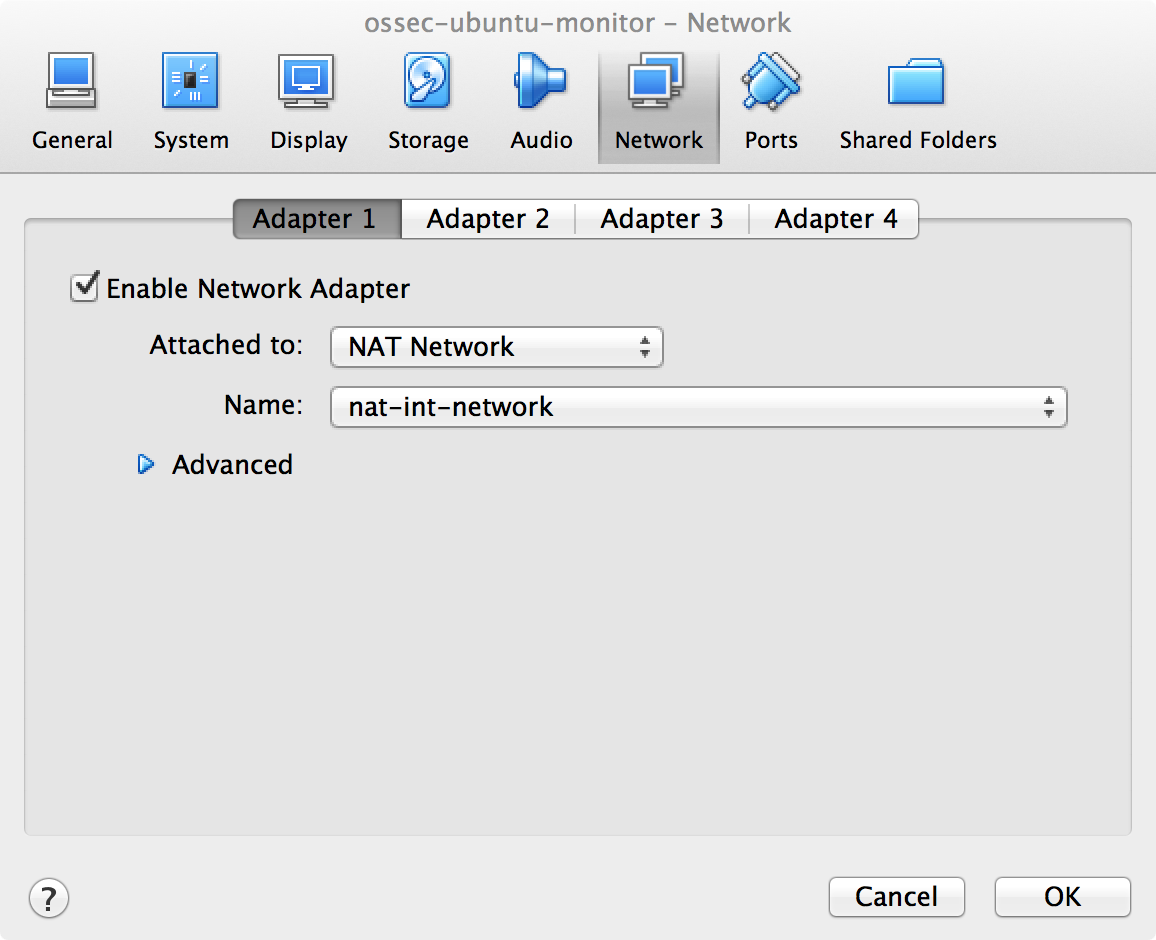
\includegraphics[scale=0.3]{pics/vbox_network_config.png}
\end{figure}


\section{Monitoring}
\subsection{Experiment overview}
To test nagios \cite{nagios:2013}, I will test the detection of
application and system failure. To test the application failure, I
will write an example application that fails after
2 minutes. I will test the system failure by inducing a kernel panic.
When an application failure is detected I will execute a script on the
cluster node to restart the application.
When a system failure is detected, I will restart the virtual
machine. 

\subsection{Nagios experiment}
I cloned the base virtual machine as described earlier and changed its
hostname to 'monitor' (by editing $/etc/hostname$ and $/etc/hosts$ and
rebooting).

On this machine, I installed nagios:
\begin{lstlisting}[language=bash]
 sudo apt-get install nagios3
\end{lstlisting}
During this installation a couple of questions were asked:
\begin{itemize}
\item email configuration: since I will not use this in my experiment
  I did not provide a configuration 
\item the nagios web administration password
\end{itemize}
In order to be able to access the web server, I opened port 80 of the
machine's firewall. 
I first enabled the UFW firewall:
\begin{lstlisting}[language=bash]
  sudo ufw enable
\end{lstlisting} 
Then I opened port 80:
\begin{lstlisting}[language=bash]
  sudo ufw allow 80/tcp
\end{lstlisting} 
Since the NAT network setup does only allow virtual machines to access
other virtual machines, I started my Windows virtual machine and used
the web browser to access the nagios system. After providing the
username and password, the browser showed the un-configured website as
depicted in \cref{fig:nagios_1}.

\begin{figure}[h!]
  \caption{Nagios start page, immediately after installation.}
  \label{fig:nagios_1}
  \centering
    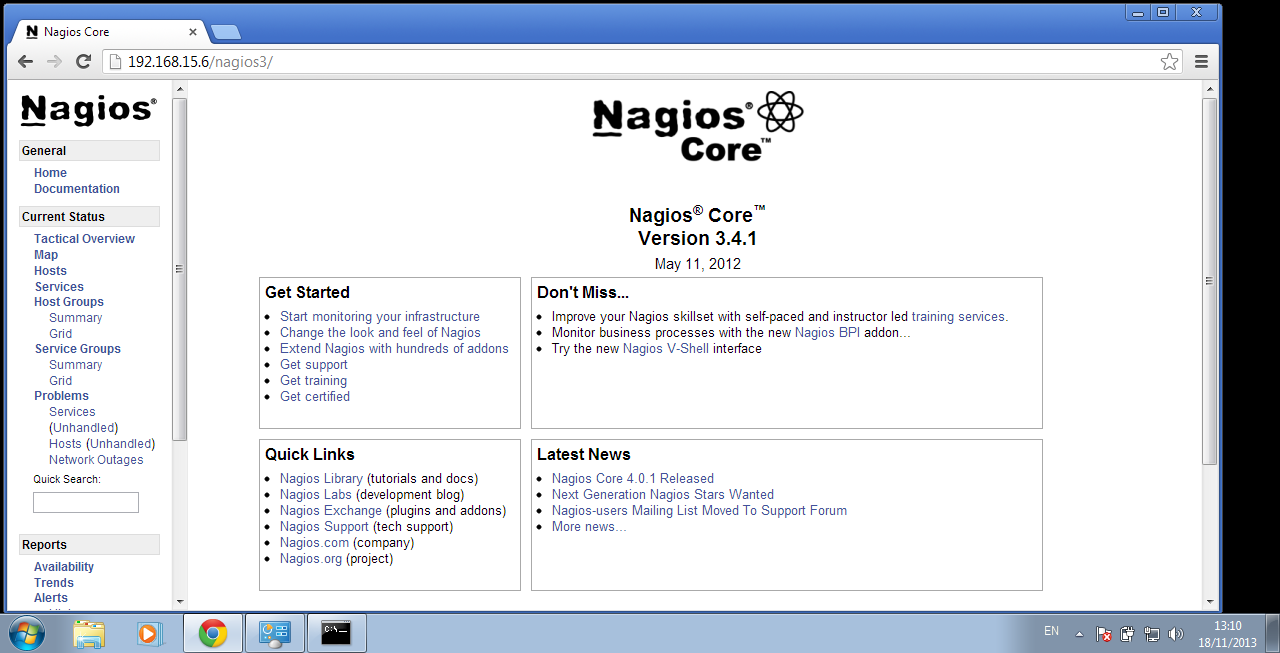
\includegraphics[scale=0.3]{pics/nagios_1.png}
\end{figure}

I cloned another pair of servers: 'node1' and 'node2', that will serve as
cluster nodes (I performed the same steps as on 'monitor' to change
the hostnames of these nodes).\\

To test the detection of application failure, I wrote a program that
fails after 2 minutes. \\

The source code of this program can be found in src/nagios/nagios\_app.cpp.
I install it on 'node1' simply by building the source code:
\begin{lstlisting}[language=bash]
  g++ nagios_app.cpp -o nagios_app 
\end{lstlisting} 
After building the application, I copy it to $/usr/sbin/$.
\footnote{In order to build this C++ code, we need gcc, this is included
in the package build-essential, which I installed earlier}

In order to start/stop and restart the service, I create an init.d
configuration script.
I based this script on the code I found on this website: 
http://koo.fi/blog/2013/03/09/init-script-for-daemonizing-non-forking-processes/
I included the source code of the nagios\_app init.d config script in src/nagios/init.d/nagios\_app.
Now we still need to give the script the correct permissions:
\begin{lstlisting}[language=bash]
  sudo chmod 755 /etc/init.d/nagios_app
\end{lstlisting} 
And we need to include it in the startup list:
\begin{lstlisting}[language=bash]
  sudo update-rc.d myscriptname defaults
\end{lstlisting}

We now can start/stop the program very easily:
\begin{lstlisting}[language=bash]
  sudo /etc/init.d/nagios_app start
  sudo /etc/init.d/nagios_app stop
\end{lstlisting}

To monitor a remote server I use the NRPE plugin for Nagios. 
This can be easily installed on the server using this command:
\begin{lstlisting}[language=bash]
  sudo apt-get install nagios-nrpe-plugin
\end{lstlisting} 

To allow nagios to detect the installation of the plugin, we need to
restart apache:
\begin{lstlisting}[language=bash]
  sudo /etc/init.d/apache2 restart
\end{lstlisting} 

On the server that is to be monitored ('node1'), we need to install the NRPE
daemon, so that the Nagios server can communicate with the remote
server
\begin{lstlisting}[language=bash]
  sudo apt-get install nagios-nrpe-server
\end{lstlisting} 

We can check whether the NRPE plugin can connect to 'node1', with this command:
\begin{lstlisting}[language=bash]
  /usr/lib/nagios/plugins/check_nrpe -H 192.168.15.4
\end{lstlisting} 
Upon the first try, I got this error message: ``Could not complete SSL
handshake''.
I was able to solve this problem by adding the server's IP address to
the list of allowed hosts in the NPRE config file
(/etc/nagios/nrpe.cfg) on 'node1'.
After restarting the NRPE daemon on 'node1', the test worked as
expected.

Now let's configure 'monitor' to monitor the general health and CPU load of  'node1'.

I added a host and service configuration to the
$/etc/nagios3/commands.cfg$ configuration file:
\begin{lstlisting}[language=bash]
define host {
        use             generic-host
        host_name       node1
        address         192.168.15.4
}

define service {
        use                     generic-service
        host_name               node1
        service_description     CPU Load
        check_command           check_nrpe!check_load
}
\end{lstlisting}
After making these changes I restarted apache.

I based all the previous actions on the official NRPE documentation
\cite{nrpe_doc}, unfortunately, this did not result in Nagios adding
the service to the list of monitored services.

After some research, I found another tutorial
\cite{nrpe_config_tutorial},
this tutorial mentioned I had to perform a reload of the Nagios
service:
\begin{lstlisting}[language=bash]
  /etc/init.d/nagios reload 
\end{lstlisting} 
This command (followed by a restart of apache), allowed Nagios to
detect the new service.
However, Nagios was not able to collect any information from this
service. I tested the command via the command line:
\begin{lstlisting}[language=bash]
  /usr/lib/nagios/plugins/check_nrpe -H 192.168.15.4 -c check_load
\end{lstlisting} 
The execution of this command resulted in the expected output, 
so I understood the problem had to be related to the nagios
configuration.
I searched for the problem, and found a post on stackoverflow.com
\cite{stackoverflow_nagios},
that mentioned the same problem as I ran into. 
The solution for this problem was explicitly instructing Nagios to
use the $check\_nrpe$ command that only accepts 1 argument.
The problem was solved after changing the configuration file like this:
\begin{lstlisting}[language=bash]
define host {
        use             generic-host
        host_name       node1
        address         192.168.15.4
}

define service {
        use                     generic-service
        host_name               node1
        service_description     CPU Load
        check_command           check_nrpe_1arg!check_load
}
\end{lstlisting}
After reloading Nagios and restarting apache, Nagios correctly fetched data
on the CPU load of 'node1' as depicted in
\cref{fig:nagios_nrpe_working_check_load}.

\begin{figure}[h!]
  \caption{Nagios showing the ``Check load'' service}
  \label{fig:nagios_nrpe_working_check_load}
  \centering
    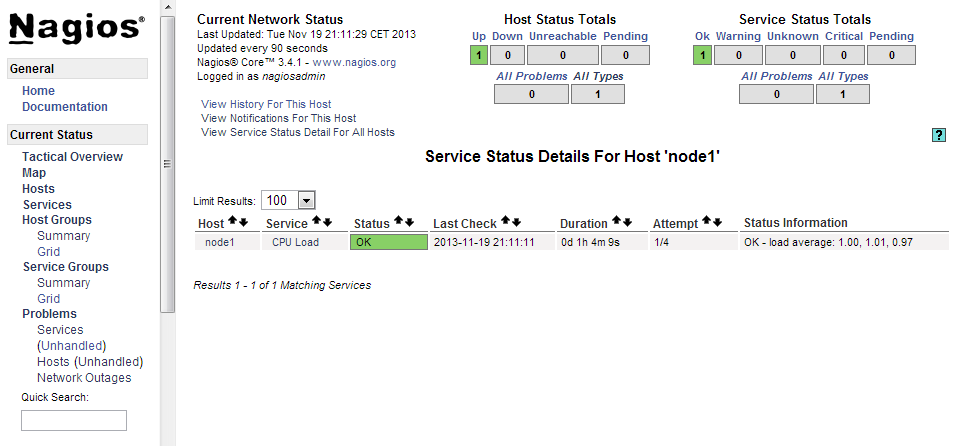
\includegraphics[scale=0.3]{pics/nagios_2.png}
\end{figure}

To do some more involved tests, I added a new node (which I called
'node2') to my list of virtual machines. I configured this machine in
the same way as I did on 'node1' and added it to the Nagios monitor
server, as described earlier.
This worked without any problems, and Nagios correctly shows the health
and CPU load of both servers 
\cref{fig:nagios_nrpe_also_node2}.

\begin{figure}[h!]
  \caption{Nagios showing both nodes}
  \label{fig:nagios_nrpe_also_node2}
  \centering
    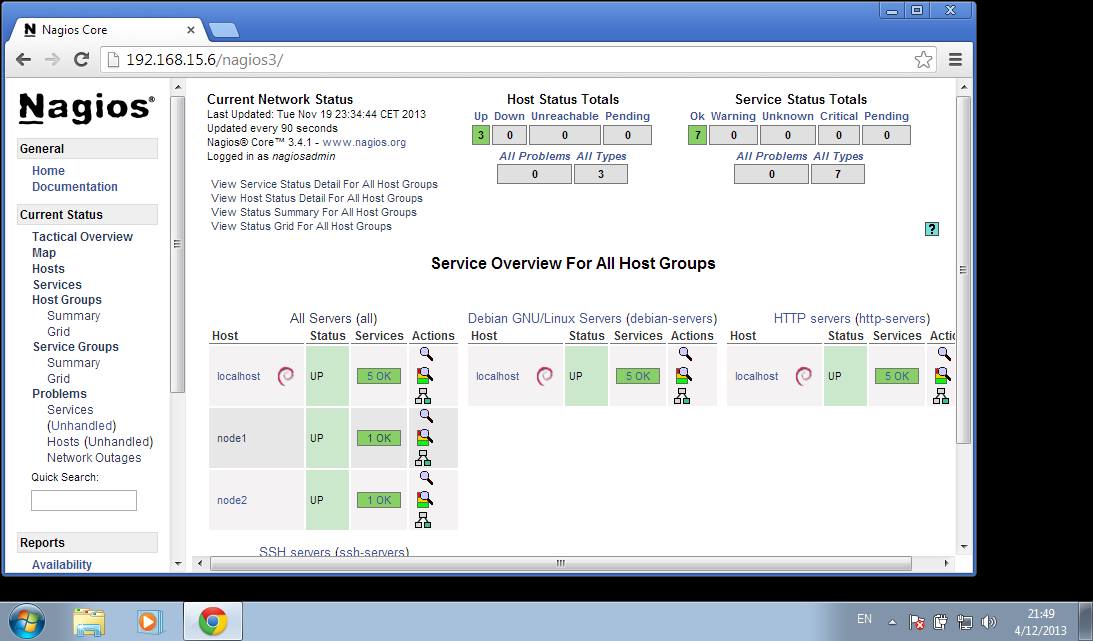
\includegraphics[scale=0.3]{pics/nagios_3.png}
\end{figure}

Now, let's see how Nagios properly detects system failure. To test
this, we will induce a kernel panic on 'node1'; this can be achieved
by inserting a kernel module that calls the panic() kernel function in
its init function. I found source code to achieve this (this code can
be found in src/panic/) \cite{simulate_linux_crash}.
To make the kernel crash, first we need to build the module:
\begin{lstlisting}[language=bash]
 make
\end{lstlisting} 
Now we can insert the module into our running kernel:
\begin{lstlisting}[language=bash]
 sudo insmod force_panic.ko
\end{lstlisting} 
This immediately causes a kernel panic (see \cref{fig:kernel_panic}).
\begin{figure}[h!]
  \caption{'node1' experiencing a kernel panic}
  \label{fig:kernel_panic}
  \centering
    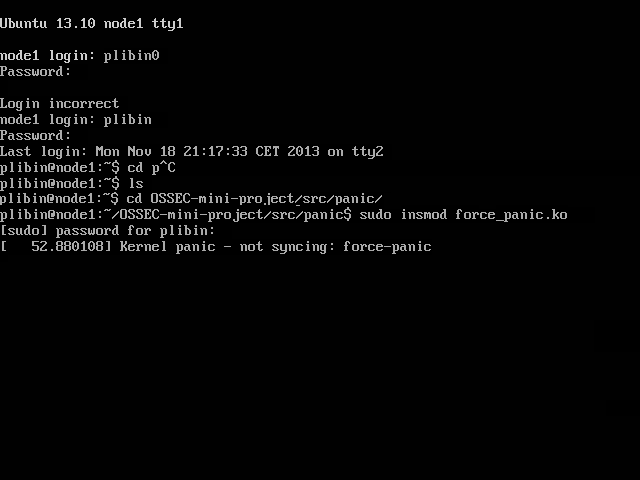
\includegraphics[scale=0.4]{pics/kernel_panic.png}
\end{figure}
After about one minute, this failure was detected by nagios, and the
user interface depicted a ``Critical error'' (see \cref{fig:nagios_after_kernel_panic}).

\begin{figure}[h!]
  \caption{Nagios showing a critical error after a kernel panic}
  \label{fig:nagios_after_kernel_panic}
  \centering
    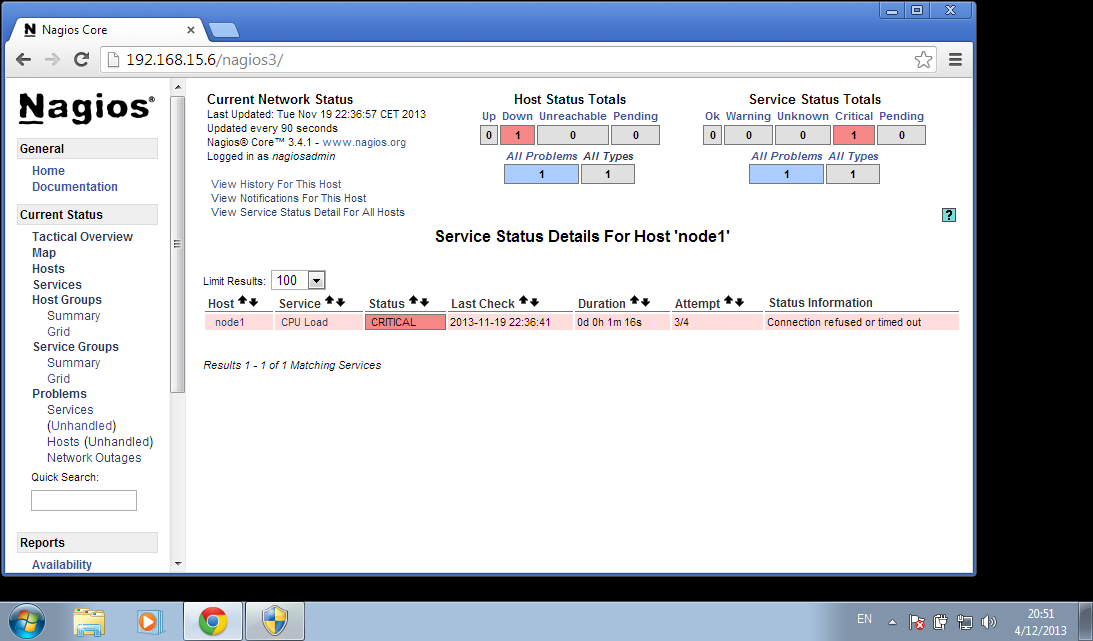
\includegraphics[scale=0.3]{pics/nagios_after_kernel_panic.png}
\end{figure}

If a node experiences a system failure, it is useful when an action is
performed that tries to solve the problem. An Ubuntu server can be
configured to automatically restart upon a kernel panic
\cite{restart_upon_kernel_panic}, however, when a hardware problem is
the cause of the system crash, restarting the node will be of no
avail. It is better to start a new node, and investigate the problem
on the crashed node in detail.

It is possible to configure an event handler for a Nagios
service. This handler will execute a script on the monitor
server, every time an exceptional event occurs.
For our simulation, we will execute this scenario:
\begin{itemize}
\item crash 'node1'
\item Nagios will notice this crash and an event handler will be
  triggered
\item this event handler will send a message to the virtual machine
  controller (in our setup, this is my MacOS X operating
  system)
\item when the controller receives this message, it will start 'node2'
\end{itemize}
Sending a message will be implemented as writing a file to a shared
directory \footnote{Shared between my MacOS X, 'node1', 'node2' and 'monitor}. This directory has the following layout:
\begin{lstlisting}[language=bash]
 ./nodes/node1
 ./nodes/node2
\end{lstlisting} 
First let's define an event handler that places a file named 'crash' in the
shared directory $./nodes/node1/$ whenever Nagios detects a critical
error.
For this to work we need to configure an event handler connected to
the host, we can do this by adding this line to the host definition ($/etc/nagios3/commands.cfg$ ) of 'node1':
\begin{lstlisting}[language=bash]
event_handler   inform-controller
\end{lstlisting} 
We now have to define the $inform-controller$ command:
\begin{lstlisting}[language=bash]
define command {
    command_name    inform-controller
    command_line    /soft/nagios/scripts/inform-controller.sh
$HOSTNAME$ $HOSTSTATE$
}
\end{lstlisting} 
The script inform-controller simply creates a file
$/media/sf\_ossec\_vm\_share/nodes/node1/crash$ whenever Nagios
detects 'node1' goes down.
Find the code for the inform-controller.sh script in src/vm\_controller/inform-controller.sh.

Now we need to detect the creation of the file
$/media/sf\_ossec\_vm\_share/nodes/node1/crash$  on the controller,
which is a MacOS X system in my testing environment. On MacOS X, this
can be implemented using ``Folder actions'', with some customised scripts
\cite{folder_actions_bash} it is possible to execute bash scripts when
an file event occurs.
I configured my MacOS X operating system to run this script whenever a
file was added to one of the node directories.
This script will check whether a crash file exists in the $./nodes/node1$
directory, and if this is the case, start 'node2' using VirtualBox's
command line tools \footnote{Source of the script: src/FolderActions.sh}

This simple setup shows how Nagios can be used to react on the failure
of cluster nodes. Note that an actual setup might be more
involved; we would for example keep a pool of available systems that
can be started when one of the running cluster nodes fails. In a
cluster environment, our VBoxManage call might be replaced with a
command to direct a hardware controller to power on an available rack
server.

I recorded a video to demonstrate this experiment:\\ 
https://www.youtube.com/watch?v=Hwzlyl\_FoZM
\\


\subsection{Ganglia experiment}
I will use the same set of virtual machines to setup the Ganglia
experiment: 'node1', 'node2' and 'monitor'.
The 'monitor' node will periodically ask the client nodes for their
metrics and store these metrics in a round-robin database.
To install the software required for this monitoring (gmetad) we execute the
following command:
\begin{lstlisting}[language=bash]
sudo apt-get install ganglia-monitor gmetad
\end{lstlisting} 

These programs only include the monitoring system, in order to
visualise the results in a web interface we should also install the
web-frontend:
\begin{lstlisting}[language=bash]
sudo apt-get install ganglia-webfronted
\end{lstlisting} 

Ganglia supports 2 modes: multicast and unicast.
The multicast is the default mechanism, and is the easiest way to
configure a Ganglia cluster.
For our test setup, where we have an explicit monitor server, we will
configure Ganglia using unicast mode.

Let's start by configuring the 'monitor' cluster node. I adapted the
default configuration file that was installed with Ganglia based on an
 installation manual \cite{ganglia_install_manual}.
Find a listing of the most important changes I've made in
src/ganglia/ganglia\_monitor\_config

The most important segments of this configuration listing are:
\begin{itemize}
\item $deaf = no$: the monitor server should listen to the cluster
  nodes
\item cluster name
\item channel (UDP/TCP) configurations
\end{itemize}

To configure the cluster nodes, we only need to install ganglia-monitor:
\begin{lstlisting}[language=bash]
sudo apt-get install ganglia-monitor
\end{lstlisting} 

I adapted the
default configuration file that was installed with Ganglia based on an
 installation manual \cite{ganglia_install_manual}.
Find a listing of the most important changes I've made in
src/ganglia/ganglia\_node\_config

The most important segments of this configuration listing are:
\begin{itemize}
\item $deaf = yes$: the cluster nodes should not listen to other
  cluster nodes, but only send their data to the monitor server
\item cluster name
\item channel (UDP) configuration
\end{itemize}

To finalise the configuration, we need to configure gmetad on
'monitor', we can do this by providing gmetad with this config file
(located at /etc/ganglia/gmetad.conf):
\begin{lstlisting}[language=bash]
data_source "OSSEC" localhost
\end{lstlisting} 

To allow the cluster nodes to send their data to the monitor server,
we still need to open the UDP port $gmetad$ is listening on:
 \begin{lstlisting}[language=bash]
sudo ufw allow 8649/udp
\end{lstlisting} 

OK, let's take it for as spin! When trying to access the web
application, there was a problem, Apache was not aware of the ganglia
web application. After copying Ganglia's Apache configuration to
$/etc/apache2/sites-enabled$, the web application was functional and
shows a general overview (\cref{fig:ganglia_general}).
\begin{figure}[h!]
  \caption{Ganglia's general overview}
  \label{fig:ganglia_general}
  \centering
    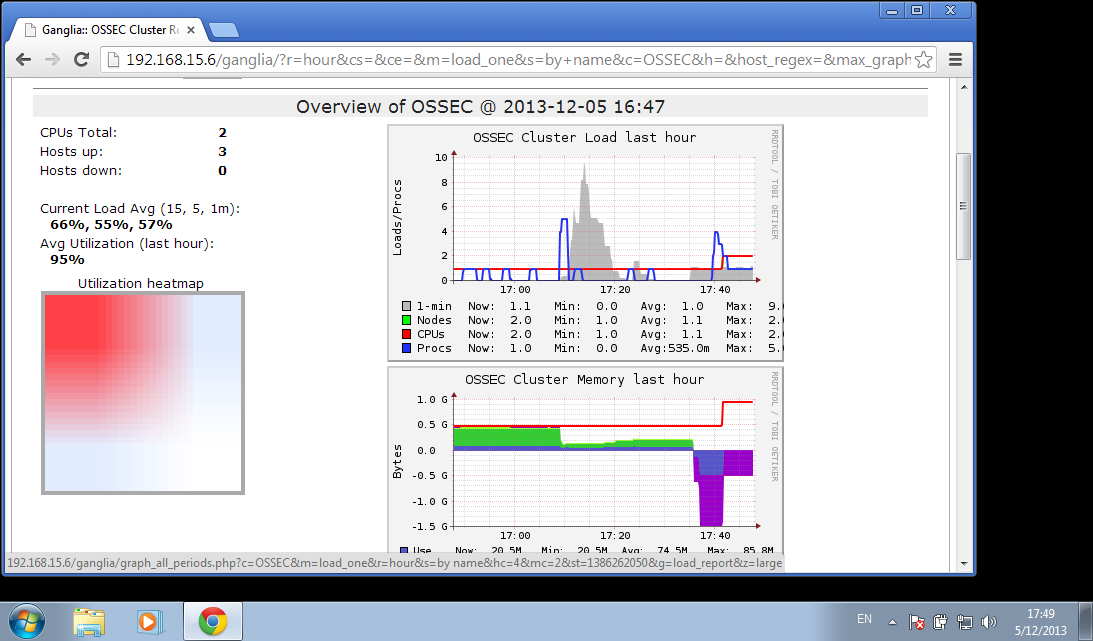
\includegraphics[scale=0.3]{pics/ganglia_general.png}
\end{figure}
All configured nodes were detected, and an overview of the CPU load of
all 3 nodes was visible on the bottom of the Ganglia's web application
start page  \cref{fig:ganglia_node_overview}.
\begin{figure}[h!]
  \caption{Ganglia's node overview}
  \label{fig:ganglia_node_overview}
  \centering
    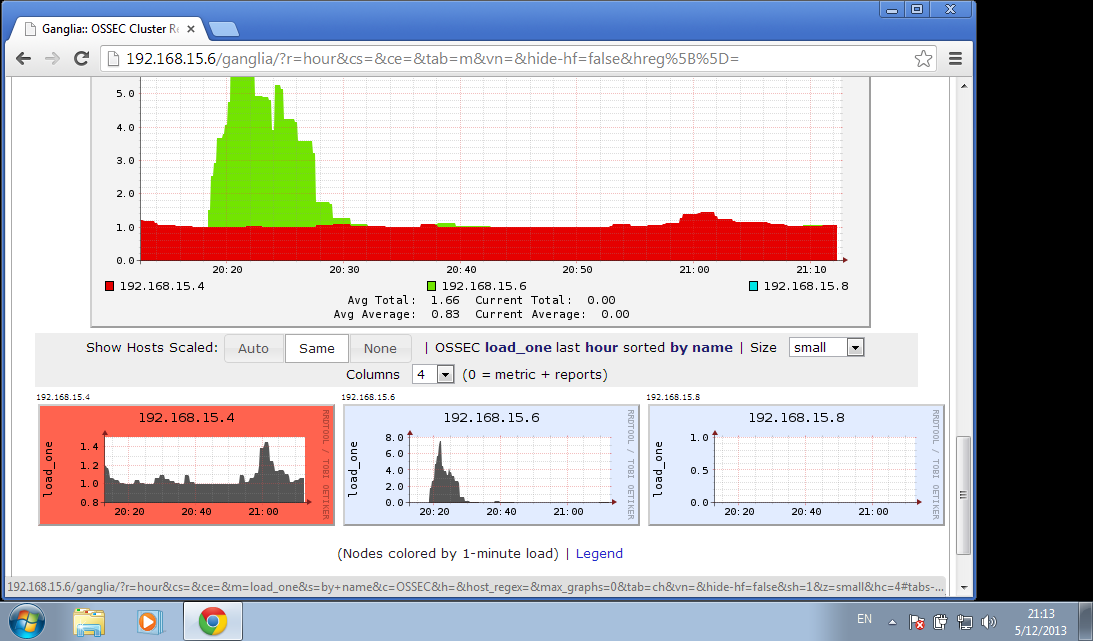
\includegraphics[scale=0.3]{pics/ganglia_node_overview.png}
\end{figure}
I've started nagios\_app (reference to the previous section) on 'node1'
(IP=192.168.15.4) to put the node under heavy load. This is
visible in the node overview (\cref{fig:ganglia_node_overview}).\\

Since the collected metrics are stored in a round-robin database, it is possible to
extract this data to do research on it. Such research can help
companies to predict/anticipate sudden changes in system load.\\

All data is stored in $/var/lib/ganglia/rrds/$, for each cluster,
there is a directory. In a cluster directory, each node that belongs
to the cluster has a directory with its name/IP address.
For example: if we want to look at the CPU user-usage of our 'node1',
we need to query this file:
$/var/lib/ganglia/rrds/OSSEC/192.168.15.4/cpu\_user.rrd$. This file is
encoded in a binary format; we can export it to a CSV-file using the
rrd2csv program \cite{rrd2csv}:
\begin{lstlisting}[language=bash]
perl rrd2csv.pl  
  /var/lib/ganglia/rrds/OSSEC/192.168.15.4/cpu_user.rrd 
  > node1_cpu_user.csv
\end{lstlisting} 

However, this command will only export the data of the last minute. To
export all data that was collected starting from a point further in time, we need to
explicitly pass the start date in epoch format.
An example to extract all data that is one hour old:
\begin{lstlisting}[language=bash]
now = `date +%s`
one_hour_ago = `expr $now - 3600` 
perl rrd2csv.pl -start $one_hour_ago 
  /var/lib/ganglia/rrds/OSSEC/192.168.15.4/cpu\_user.rrd 
  > node1_cpu_user.csv
\end{lstlisting} 

This kind of data (in CSV format) can be imported directly by statistical analysis
environments such as R \cite{r_software}.

\subsection{Nagios and Ganglia: evaluation}
Both systems are very interesting and mostly complementary.
\subsubsection{Nagios}
Nagios has a very powerful component: the event handler .This system makes it
possible to react on failures. The software is very
extensible and configurable.\\
Some negative remarks: 
\begin{itemize}
\item the documentation is not always up to date and sometimes incomplete
\item the installation was difficult (largely
  because of the bad quality of the documentation)
\item the installation required a lot of manual configurations,
  maybe it would be better that some working default configuration was
  in place (to give users a working starting point)
\end{itemize}
\subsubsection{Ganglia}
The installation was easy; apt-get did almost everything. The
configuration that was required to enable unicast was not that
difficult to perform (the documentation is in good shape and this helped a lot).
Collected data is stored in a round-robin database by default, this is
positive, since there exists already a lot of software packages
to query/extract/graph data from such databases.

\section{HAProxy experiment}
\label{ha_proxy_experiment}
HAProxy is a prominent software load balancer. It acts like a reverse
proxy; pretending it is the main server and then forwarding the
requests to one of the HTTP server cluster nodes.
Several strategies are available to distribute requests over a HTTP
server cluster; these strategies are explained in
\cref{sec:load_balancing_proxies}.
In this experiment, I will setup a HAProxy that sends requests to 2
HTTP server cluster nodes using the 'round robin' distribution
strategy.
\subsection{HAProxy installation}
I will install HAProxy on a new Ubuntu virtual machine: 'haproxy'.
I will use the virtual machines 'node1' and 'node2' as HTTP server cluster nodes.
Let's start by properly configuring 'node1' and 'node2' that it can
serve this simple PHP program (from \cite{haproxy_install_tutorial}):
\label{lst:test_php}
\begin{lstlisting}[language=php]
<?php
header('Content-Type: text/plain');
echo "Server IP: ".$_SERVER['SERVER_ADDR'];
echo "\nClient IP: ".$_SERVER['REMOTE_ADDR'];
echo "\nX-Forwarded-for: ".$_SERVER['HTTP_X_FORWARDED_FOR'];
?>
\end{lstlisting} 
This program will print the HTTP server's IP address, the client IP
address (which in our case will be the IP address of our HAProxy
server) and the X-Forwarded-for header (which will allow us to identify
the originating IP address: i.e. the IP-address of our browser).
First we'll need to install Apache and PHP:
\begin{lstlisting}[language=bash]
sudo apt-get install apache2
sudo apt-get install php5
sudo apt-get install libapache2-mod-php5
sudo /etc/init.d/apache2 restart
\end{lstlisting} 
Now we can copy our test program \cref{lst:test_php} to
$/var/www/test.php$.

Then I opened port 80:
\begin{lstlisting}[language=bash]
  sudo ufw allow 80/tcp
\end{lstlisting} 

After these changes, the nodes were able to serve this PHP test
program: \cref{fig:test_php_working}.

\begin{figure}[h!]
  \caption{Test PHP program working in a browser}
  \label{fig:test_php_working}
  \centering
    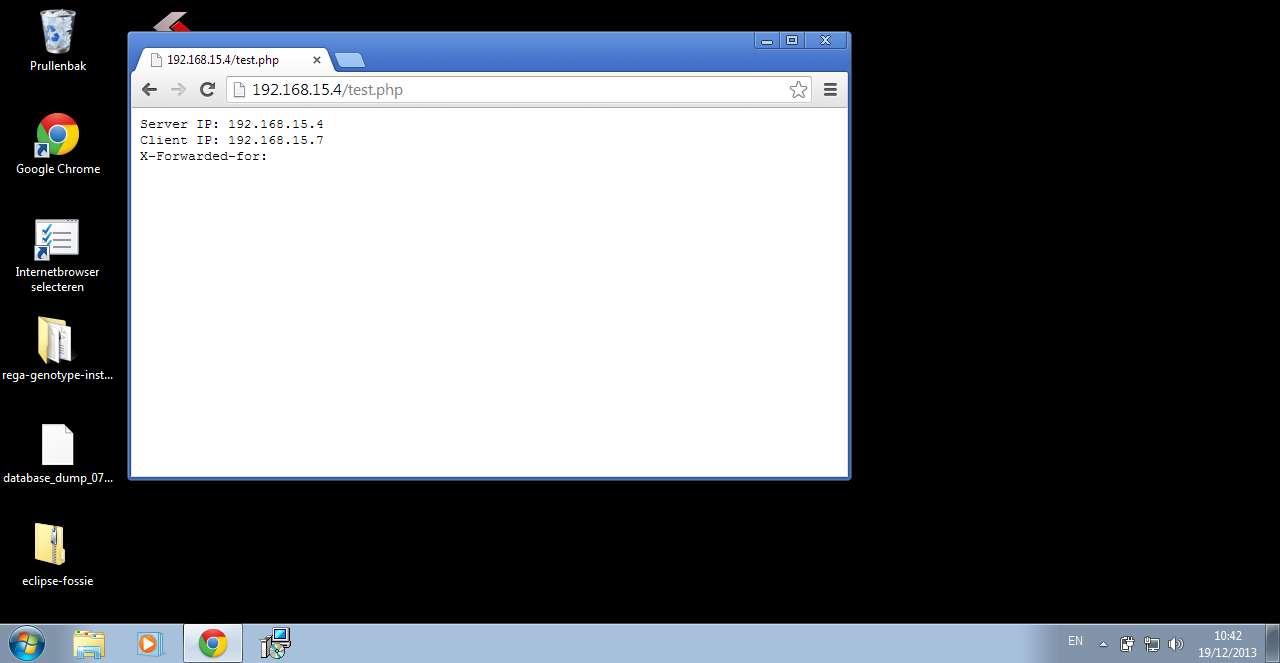
\includegraphics[scale=0.3]{pics/test_php_working.png}
\end{figure}

To install HAProxy:
\begin{lstlisting}[language=bash]
apt-get install haproxy
\end{lstlisting} 
After this installation, a reboot of the virtual machine was required.
In order to make HAProxy start by the init script we need to put the
ENABLED variable in $/etc/default/haproxy$ to $1$.
The haproxy
Ubuntu package comes with a proper config file by default (in src/haproxy/haproxy-basic.cfg).   
In order to configure HAProxy for this specific application, I conceived
this configuration snippet (the full config file can be found in src/haproxy/):
\begin{lstlisting}[language=bash]
listen ossec_app 0.0.0.0:80
        mode http
        balance roundrobin
        option forwardfor
        server node1 192.168.15.4:80 check
        server node2 192.168.15.8:80 check
\end{lstlisting} 
This configuration defines the application ossec\_app on port 80.
I selected the 'roundrobin' algorithm, enabled the forwardfor (so we can read
the X-Forwarded-for HTTP header in our PHP test program) and added our 2
HTTP server cluster nodes to the configuration.
Then I opened port 80 on the 'haproxy' server:
\begin{lstlisting}[language=bash]
  sudo ufw allow 80/tcp
\end{lstlisting} 

\subsection{HAProxy testing}
After making the configurations as described in the previous section, I could visit the test PHP program via the
haproxy server (IP address: 192.168.15.10); as demonstrated in 
\cref{fig:haproxy_working_browser}.

\begin{figure}[h!]
  \caption{Testing the haproxy setup in a browser}
  \label{fig:haproxy_working_browser}
  \centering
    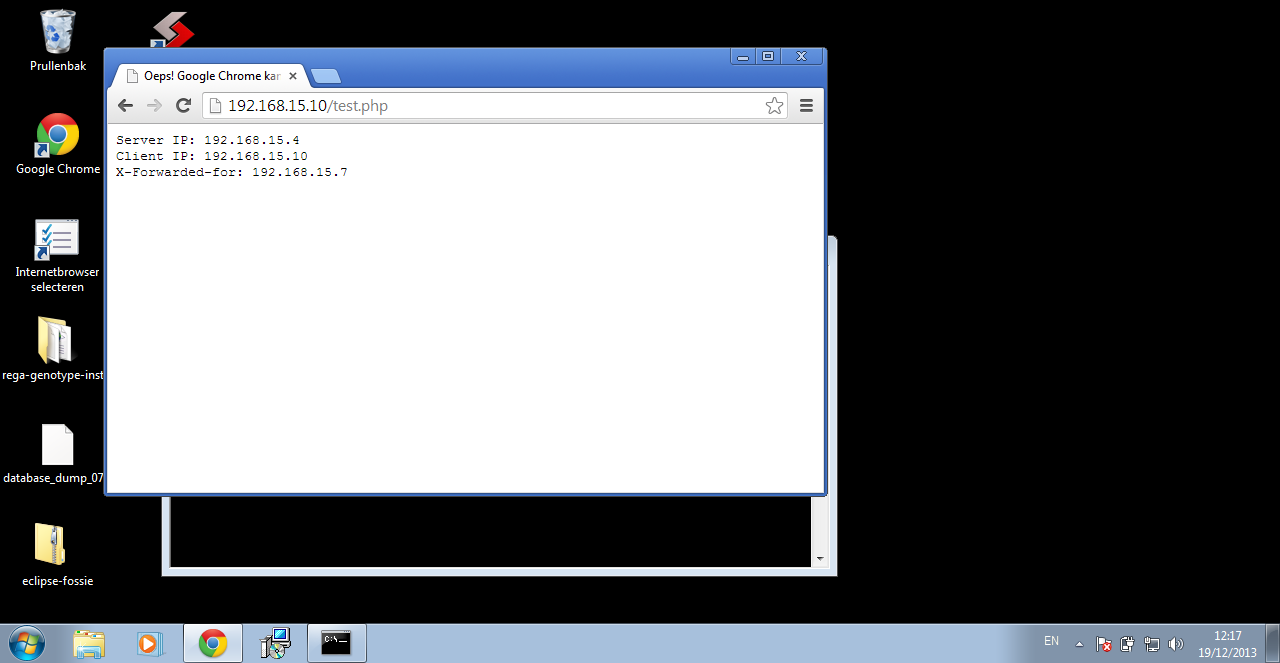
\includegraphics[scale=0.3]{pics/haproxy_working_browser.png}
\end{figure}

When testing this setup, it becomes clear that HAProxy forwards the
request to both cluster nodes (subsequently to 'node1' and than to
'node2').\\
I recorded a video to demonstrate this experiment: \\
https://www.youtube.com/watch?v=hrjdLpFLEDM \\

This setup also handles failure of nodes, if we shutdown apache on one
of the nodes, HAProxy will automatically forward the incoming requests
to the working node. \\
I also recorded a video to demonstrate this: \\
https://www.youtube.com/watch?v=ME9HS\_r6nZg

\subsection{Conclusion and remarks}
I was able to extract a lot of valuable information from this online
article: \cite{haproxy_install_tutorial}. The online documentation of
 HAProxy \cite{haproxy:2013} is also very good, and explains all
 configuration items in detail, often with some pointers on when an
 how to use them. The documentation for example advices not to use the
 'leastconn' algorithm for HTTP services, since this algorithm is not
 well-suited for services that use short-lived sessions.
The installation went smoothly on Ubuntu, some manual configurations
were necessary, but since the documentation of the project is clear
and up-to-date, this did not cause any problems.

\section{Database replication experiment}
I will setup a master-slave replicated MySQL database. I will use the
'haproxy' virtual machine to act as my master database and I will
install 2 slave databases on my 'node1' and 'node2' virtual machines.
I used the following documentation and tutorials:
\cite{mysql_official_replication_doc}, \cite{mysql_replication_howtoforge}, \cite{mysql_replication_stackexchange}.

\subsection{Installation} 
I will start by installing mysql (server and client) on all the involved virtual
machines ('haproxy','node1','node2').
\begin{lstlisting}[language=bash]
sudo apt-get install mysql-server mysql-client
\end{lstlisting}

Let's create a test database on our master-node:
\begin{lstlisting}[language=bash]
mysql -u root -p
*type password*
mysql> CREATE DATABASE ossec;
\end{lstlisting}
No we can use this database, and create a simple table in it:
\begin{lstlisting}[language=bash]
mysql> USE ossec;
mysql> CREATE TABLE friend (first_name text, last_name text);
\end{lstlisting}
And we add a friend to it:
\begin{lstlisting}[language=bash]
mysql> INSERT INTO friend (first_name, last_name) values ('Eric',
'Northman');
\end{lstlisting}

The next step is the configuration of the master. Most of the
configuration is done in $/etc/mysql/my.cnf$.
First we need to comment out the bind-address line, this will inform MySQL
to listen on all IP addresses rather than only on localhost:
\begin{lstlisting}[language=bash]
#bind-address        = 127.0.0.1
\end{lstlisting}
MySQL slaves use the logs that a master-node generates to replicate
the database. In order to make this work, we need to tell the MySQL
master-node where to
generate these log files and for which databases the log files need to
be generated. 
\begin{lstlisting}[language=bash]
log-bin = /var/log/mysql/bin.log
#multiple binlog-do-db lines are allowed
binlog-do-db = ossec
\end{lstlisting}
We need to specify the server's id as well, since this is our master
server, we use $id=1$:
\begin{lstlisting}[language=bash]
server-id = 1
\end{lstlisting}
Now we're ready for restarting the database:
\begin{lstlisting}[language=bash]
sudo /etc/init.d/mysql restart
\end{lstlisting}
We need to give a MySQL user (let call him 'reppy') the permission to replicate our
database:
\begin{lstlisting}[language=bash]
mysql -u root -p
*type password*
mysql> GRANT REPLICATIOn SLAVE ON *.* TO 'reppy'@''%' 
       IDENTIFIED BY 'reppy_password';
mysql> FLUSH PRIVILEGES;
\end{lstlisting}
The \% in this command allows the user to login from any IP address.\\

To get the information to configure the slave, we need to execute these
commands to select our database 'ossec' and lock all the tables in it:
\begin{lstlisting}[language=bash]
mysql> USE ossec;
mysql> FLUSH TABLES WITH READ LOCK;
\end{lstlisting}
No we can extract the information we need:
\begin{lstlisting}[language=bash]
mysql> SHOW MASTER STATUS;
\end{lstlisting}
The output of this command is:
\begin{lstlisting}[language=bash]
+---------------+----------+--------------+------------------+
| File          | Position | Binlog_do_db | Binlog_ignore_db |
+---------------+----------+--------------+------------------+
| bin.000003    | 333      | ossec        |                  |
+---------------+----------+--------------+------------------+
1 row in set (0.00 sec)
\end{lstlisting}
Now we need to dump the current database:
\begin{lstlisting}[language=bash]
mysqldump -u root -p --opt ossec > ossec.sql
\end{lstlisting}

It is important to unlock the tables again before we continue:
\begin{lstlisting}[language=bash]
mysql> UNLOCK TABLES;
\end{lstlisting}

To allow the slave nodes to connect to the master database, we need to
open up the MySQL port ($3306$) of the master node:
\begin{lstlisting}[language=bash]
sudo ufw allow 3306/tcp
\end{lstlisting}

Now let's configure the slaves, we start by creating the 'ossec'
database on the slaves:
\begin{lstlisting}[language=bash]
mysql -u root -p
*type password*
mysql> CREATE DATABASE ossec;
\end{lstlisting}
Now we need to apply the dump we obtained on the master server (I
copied the ossec.sql using $scp$):
\begin{lstlisting}[language=bash]
mysql -u root -p ossec < ossec.sql
*type password*
\end{lstlisting}

Next we configure the server-id and the database that is replicated in
$/etc/mysql/my.cnf$:
\begin{lstlisting}[language=bash]
#on node 1
server-id = 2 
#on node 2
server-id = 3

#same for node 1 and 2
replicate-do-db = ossec
\end{lstlisting}

After these configurations, we need to restart the MySQL server:
\begin{lstlisting}[language=bash]
sudo /etc/init.d/mysql restart
\end{lstlisting}

And execute this SQL to let the slave know where to find its master:
\begin{lstlisting}[language=bash]
mysql> CHANGE MASTER TO MASTER_LOG_FILE='bin.000003',
  MASTER_LOG_POS=333, MASTER_HOST='192.168.15.10', 
  MASTER_USER='reppy', MASTER_PASSWORD='reppy_password';
\end{lstlisting}
Now we can start the slave:
\begin{lstlisting}[language=bash]
mysql> START SLAVE;
\end{lstlisting}

\subsection{Testing the experiment setup}
After this, when a change is made to the master database, these
changes are automatically propagated to the slave databases.\\
 I recorded a video to demonstrate this experiment:\\
https://www.youtube.com/watch?v=hQfTVrYzT3o\\

Another video show how 2 DRBD nodes find each other when they are
started up:\\
https://www.youtube.com/watch?v=DP923CWyZhM

\subsection{Conclusion and remarks}
Setting up a replicated MySQL environment was not easy, mainly since I
had to consult several separate documents (\cite{mysql_official_replication_doc}, \cite{mysql_replication_howtoforge}, \cite{mysql_replication_stackexchange}). The main problem seems to
be that the way things are configured in MySQL seems to change significantly
over time. Several settings I found in different tutorials, were no
longer supported on the most recent MySQL package distributed with
Ubuntu.
On the other hand, if something went wrong or behaved unexpectedly,
the output in the log files was quite informative. 
One important remark is that on a slave node, it is no longer possible
to configure the master settings (host, log\_pos, log\_file, user,
password) in the configuration file; you should use the $CHANGE
MASTER ...$ SQL command.

\section{Software disk replication experiment}
I will setup a network RAID-1 (mirror)
system on 2 nodes, for this I will use the software DRBD 
(Distributed Replicated Block Device) \cite{drbd_soft:2013}.
I will create a disk (virtual machine disk) of 1GB on my virtual
machines 'node1' and 'node2' (since we're using RAID, it is vital that
these disks have the exact same size).\\

I used the following documentation and tutorials:
\cite{drbd_ubuntu_doc}, \cite{drbd_official_doc}, \cite{drbd_howtoforge}.

\subsection{Adding the ``disks''}
Firstly, I will add a disk to my virtual machines 'node1' and
'node2'. This can be done via the VirtualBox user interface, when the
virtual machines are powered off \cref{fig:add_disk_vbox}.

\begin{figure}[h!]
  \caption{Added a disk to one of the virtual machines}
  \label{fig:add_disk_vbox}
  \centering
    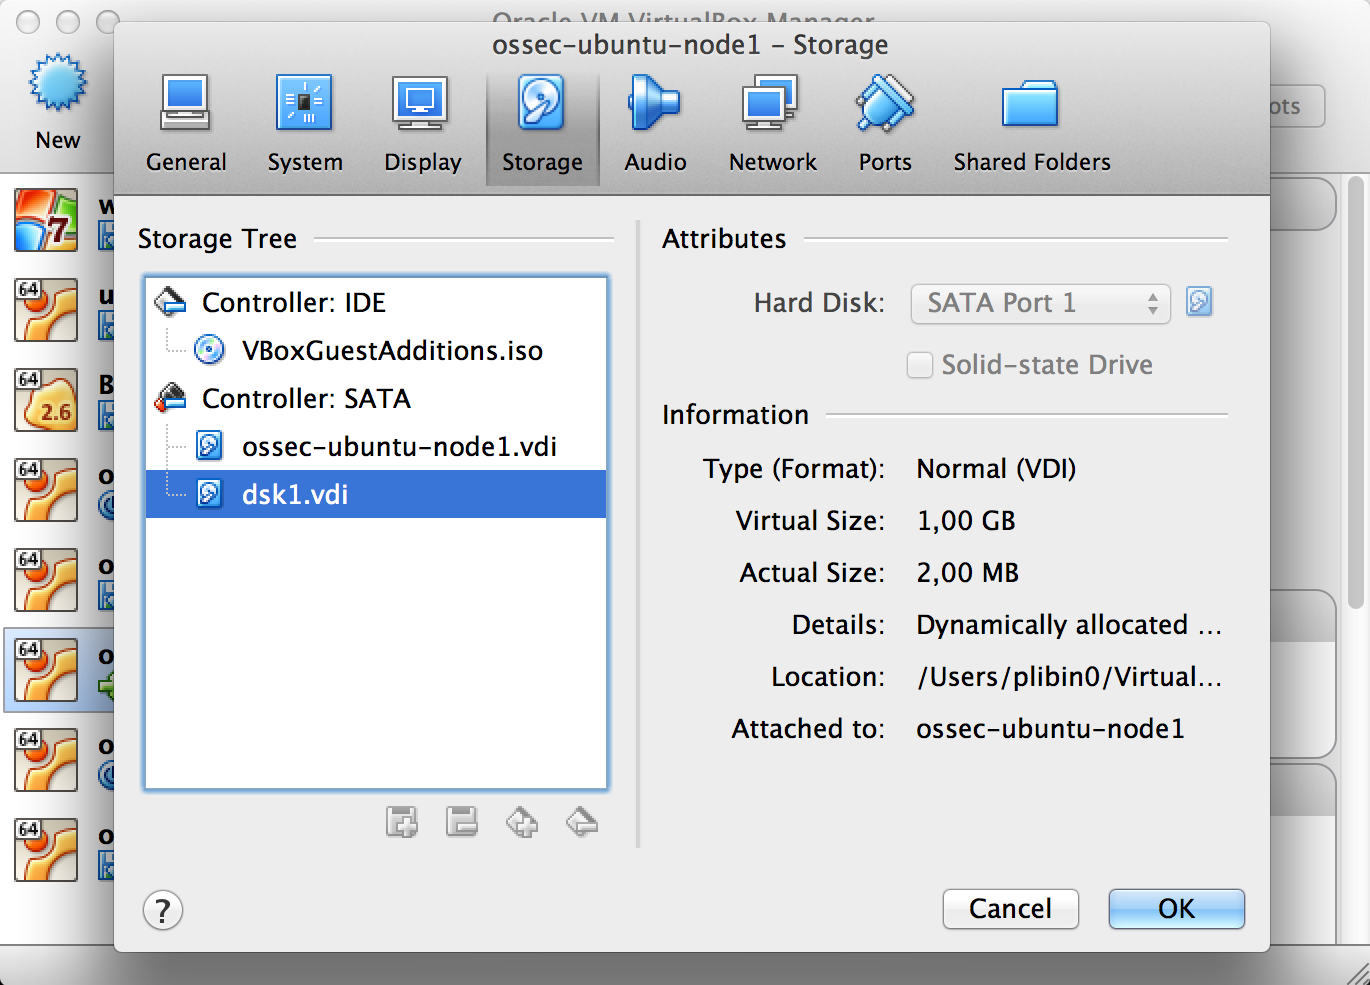
\includegraphics[scale=0.3]{pics/add_disk_vbox.png}
\end{figure}

\subsection{Setting up the network RAID-1}
To ensure the synchronisation is timed well, I will install the NTP packages.
\begin{lstlisting}[language=bash]
sudo apt-get install ntp ntpdate
\end{lstlisting}

In order for DRBD to work, each node should be able to access the
other node by name. Since we have no DNS in place, we need to
configure this in the $/etc/hosts$ config file.

We added a disk to the virtual machine, however, this disk is
currently an unpartitioned and unformatted device.
Let's first have a look at our device:
\begin{lstlisting}[language=bash]
sudo fdisk -l /dev/sdb
\end{lstlisting}
This command show the following report:
\begin{lstlisting}[language=bash]
Disk /dev/sdb: 1073 MB, 1073741824 bytes
255 heads, 63 sectors/track, 130 cylinders, total 2097152 sectors
Units = sectors of 1 * 512 = 512 bytes
Sector size (logical/physical): 512 bytes / 512 bytes
I/O size (minimum/optimal): 512 bytes / 512 bytes
Disk identifier: 0x00000000
\end{lstlisting}
To create a partition:
\begin{lstlisting}[language=bash]
sudo fdisk /dev/sdb
Command (m for help): n #create a new partition
Select (default p): p #primary partition
Partition number (1-4, default 1): 1
First sector (2048-2097151, default 2048): 2048
Last sector (2048-2097151, default 2097151): 2097151
\end{lstlisting}
The partition is created, but we still need to write the partition
table to the disk:
\begin{lstlisting}[language=bash]
Command (m for help): w #write the partition table to disk
\end{lstlisting}
When running $fdisk -l$ again, we get this output:
\begin{lstlisting}[language=bash]
Disk /dev/sdb: 1073 MB, 1073741824 bytes
139 heads, 8 sectors/track, 1885 cylinders, total 2097152 sectors
Units = sectors of 1 * 512 = 512 bytes
Sector size (logical/physical): 512 bytes / 512 bytes
I/O size (minimum/optimal): 512 bytes / 512 bytes
Disk identifier: 0x1053cb0b

   Device Boot      Start         End      Blocks   Id  System
/dev/sdb1            2048     2097151     1047552   83  Linux
\end{lstlisting}

Now we need to install the DRBD utilities:
\begin{lstlisting}[language=bash]
sudo apt-get install drbd8-utils
\end{lstlisting}
And load the DRBD kernel module:
\begin{lstlisting}[language=bash]
sudo modprobe drbd
\end{lstlisting}

We can configure these nodes with the following configuration file
(based on: \cite{drbd_ubuntu_doc} \cite{drbd_official_doc}):
\begin{lstlisting}[language=bash]
global {
       	#do NOT participate in DRBD's online usage counter:
       	#explicitely disable this, and also disable that we are
       	#asked for this on every restart of the drbd daemon
       	usage-count no;
}
resource r0 {
	net {
                #one of the 3 possible protocols: A, B, C
                #see documentation for details
		protocol C;
                #specifies the HMAC algorithm (see Appendix)
                #to enable peer authentication
		cram-hmac-alg sha1;
                #secret used in peer authentication
		shared-secret "testing";
	}
	on node1 {
		volume 0 {
			#the new device we configure
			device    /dev/drbd0;
			disk      /dev/sdb1;
			meta-disk internal;
		}
		address   192.168.15.4:7789;
	}
	on node2 {
		volume 0 {
			#the new device we configure
			device    /dev/drbd0;
			disk      /dev/sdb1;
			meta-disk internal;
		}
		address   192.168.15.8:7789;
	}
}
\end{lstlisting}
Most of the configuration items are straightforward, I commented the
other elements to clarify their meaning.
The configuration file should be placed in $/etc/drbd.conf$.

We need to open the ports 7789 on both nodes:
\begin{lstlisting}[language=bash]
sudo ufw allow 7789/tcp
\end{lstlisting}

We also need to restart the drbd daemon: 
\begin{lstlisting}[language=bash]
sudo /etc/init.d/drbd restart
\end{lstlisting}

First I started the daemon on 'node1', the daemon waited until the
daemon I brought the daemon on 'node2' online.

Now we configured the mirrored device $/dev/drbd0$, but we can't use
this device yet.
We first need to initialise the meta data storage of each physical
device,
one both nodes, we need to run this command:
\begin{lstlisting}[language=bash]
sudo drbdadm create-md r0
\end{lstlisting}
We also need to decide which node will be the primary node; on this
node we will be able to read and write data d.
For now, I will make 'node1' the primary node for this device.
First we need to invalidate the data on 'node2', so BRBD knows this
data can safely be overiden; we use this command:
\begin{lstlisting}[language=bash]
sudo drbdadm invalidate r0
\end{lstlisting}
To make the device on 'node1' the primary device,
we need to run this command on 'node1':
\begin{lstlisting}[language=bash]
sudo drbdadm --force primary r0
\end{lstlisting}
Now the device on 'node1' gets automatically synched with the one on
'node2'. But there doesn't exist a filesystem on our device yet; let's
create an ext3-filesystem (this command is executed no 'node1'):
\begin{lstlisting}[language=bash]
sudo mkfs.ext3 /dev/drbd0
\end{lstlisting}
Now we can mount the filesystem (on 'node1'):
\begin{lstlisting}[language=bash]
sudo mkdir /media/drdb0
sudo mount /dev/drbd0 /media/drbd0 
\end{lstlisting}
To test that the replication actually works, we need to:
\begin{itemize}
\item create some files on $/media/drbd0$ on 'node1'
\item unmount the $/media/drbd0$ on 'node1'
\item make 'node1' the secondary host
\item make 'node2' the primary host
\item mount the device on 'node2'
\item check that the files we placed on the device from 'node1' also
  appear on 'node2'
\end{itemize}

I recorded a video to demonstrate this experiment:\\
https://www.youtube.com/watch?v=oMCyT1wCPmA

\subsection{Conclusions and remarks}
The drdb service can send statistics (anonymized) to a
server of the DRBD organisation (to get a better overview about who is
using the software). This option is however enabled by
default, in my opinion, this should be disabled by default
\footnote{To disable this, we need to add the line ``usage-count no;''
  to the config file's global section.}.\\
The online documentation on how to configure the software is
up-to-date and helpful. It is a nice and interesting software, that easily allows you
to setup replication between data centers on block level.

\section{Distributed file system experiment}
I will experiment with Ceph, since this seems to be the de-facto
standard distributed filesystem in the Ubutu landscape.
Except for better compatibility with Ubuntu, there is no real reason
to choose Ceph over GlusterFS; both seem to be decent projects
\cite{ceph_vs_gluster_1}, \cite{ceph_vs_gluster_debate}.
Ceph is a large project, with many features: object storage, file
system, block device layer, ... In this experiment, I will focus on
the distributed object storage component.

\subsection{Architecture}
\label{subsec:ceph_architecture}
Ceph has a layered architecture as demonstrated in
\cref{fig:ceph_architecture} \cite{ceph_architecture}.

\begin{figure}[h!]
  \caption{Ceph archtitecture}
  \label{fig:ceph_architecture}
  \centering
    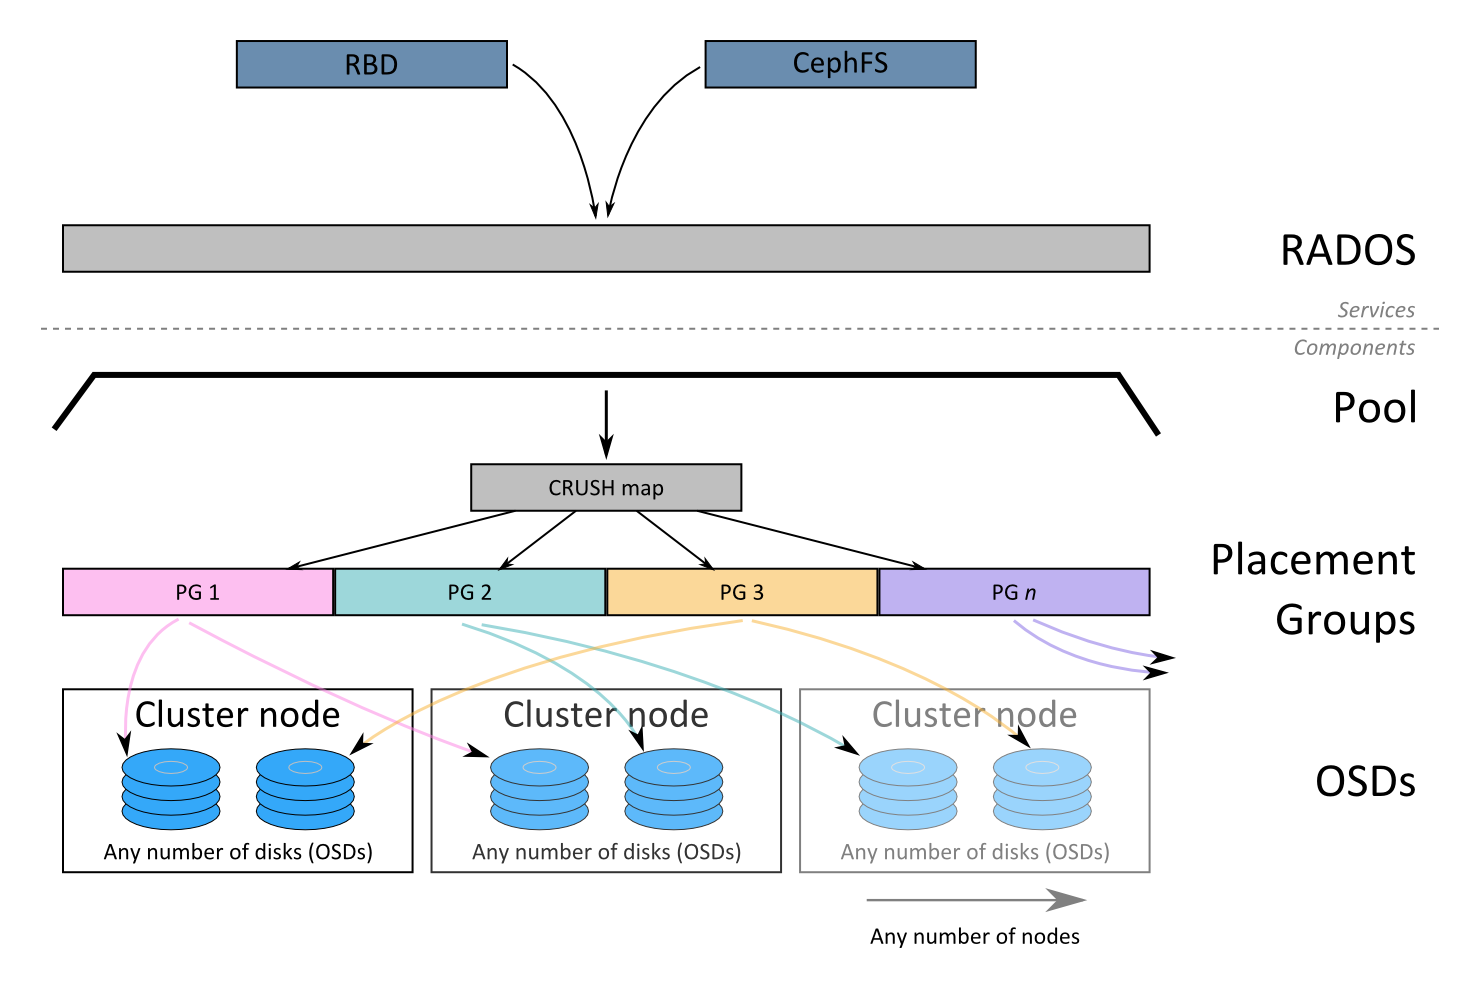
\includegraphics[scale=0.3]{pics/ceph_architecture.png}
\end{figure}

The RADOS layer allows for client software to use the cluster
infrastructure  (file systems, key value stores,... ). This layer
communicates with the cluster pool via the CRUSH layer; which
distributes objects over the different nodes in the cluster, and makes
sure that they can be fetched optimally. \\
They architecture allows for easy scaling since nodes can be added and
removed while the system is running. When such an event occurs the
CRUSH layer will automatically rebalance the objects over the cluster.

Reference: \cite{ceph_developerworks}.

\subsection{Installation}
To perform this installation I used the official Ceph documentation \cite{ceph_official_doc}.
Ceph can be installed in 2 ways: via ceph-deploy (as piece of software
that is installed on an administrator node that automatically installs the
necessary components on the nodes in your Ceph cluster) and a
manual installation.
The advantages of the first approach:
\begin{itemize}
\item it's quicker to setup
\item commands entered on the administrative node are 
  propagated to all relevant cluster nodes (this makes upgrading nodes
  much easier)
\end{itemize}
The main advantage of a manual installation is that it allows you to
fully control where and when all necessary components are installed on the different
nodes. 
This might be interesting on a production cluster, however I think the
installation via ceph-deploy is more appropriate for this experiment, since it will
allow me to test more of Ceph's features in a shorter timespan.

\subsubsection{Nodes}
We will first setup a cluster with 1 administrator node and a Ceph
Storage Cluster consisting of 3 cluster nodes (this setting is advised
by the official documentation to experiment with the software \cite{ceph_official_doc}).
For this, I create 4 new clones of my base virtual machine:
'ceph-admin', 'ceph-node1', 'ceph-node2', 'ceph-node3'.

\subsubsection{Preparation of the cluster nodes}
Ceph requires some basic stuff to be in place, in order to be able to
use ceph-deploy to configure the cluster and cluster nodes.
The instructions are well documented in the official documentation's
``Ceph node setup'' section \cite{ceph_official_doc}.
A quick overview of the different steps:
\begin{itemize}
\item create a 'ceph' user on each node
\item add root privileges to the 'ceph' user
\item install an ssh server
\item configure the admin node so that it can access the cluster nodes
  without using a password (using SSH keys)
\item all nodes should be able to access each other using hostname
  resolution, in my case, we had to update the $/etc/hosts$ file to
  make this possible, since we have no DNS server in our lab setting
\end{itemize}

\subsubsection{Configuring the ceph-admin node}
The documentation requests to add the ceph-deploy package to your
local APT
repository, however on Ubuntu 13.10, this package was already
available by default.
So we can install it like this:
\begin{lstlisting}[language=bash]
sudo apt-get install ceph-deploy
\end{lstlisting}
We also need to create a directory to maintain the configuration of
our cluster (the name is not important, but we will use
~/ossec-cluster consistently through the example for clarity):
\begin{lstlisting}[language=bash]
mkdir ~/ossec-cluster
\end{lstlisting}
It is important that we run  the ceph-deploy command in this
directory, since it will export its output to the current directory.

\subsubsection{Setting up the cluster}
Now we can start configuring our cluster \footnote{The following steps are executed on the 'ceph-admin'}.
We will configure 'ceph-node1' as a monitor node, 'ceph-node2' and
'ceph-node-3' will be object storage daemons (see \cref{subsec:ceph_architecture}).

To start a new cluster with monitor node 'ceph-node1':
\begin{lstlisting}[language=bash]
cd ~/ossec-cluster
ceph-deploy new ceph-node1
\end{lstlisting}
After executing these commands, a set of files will be created in
~/ossec-cluster.
To install ceph on our nodes:
\begin{lstlisting}[language=bash]
ceph-deploy install ceph-node1 ceph-node2 ceph-node3
\end{lstlisting}
Every Ceph cluster is required to have at least one monitor
\footnote{Multiple monitor nodes are also supported; this is vital for a high
  availability production cluster, but outside the scope of this experiment} :
\begin{lstlisting}[language=bash]
ceph-deploy mon create ceph-node1
\end{lstlisting}
To be able to add Object Storage Daemons, we need to gather the
monitor node's
keys:
\begin{lstlisting}[language=bash]
ceph-deploy gatherkeys ceph-node1
\end{lstlisting}
To add the Object Storage Daemons (OSDs), we first need to make a uniquely
named directory on the nodes. I created /opt/OSD-disk0 on ceph-node2 and
/opt/OSD-disk1 on ceph-node3. 
Now we can prepare and activate the OSDs:
\begin{lstlisting}[language=bash]
ceph-deploy osd prepare ceph-node2:/opt/OSD-disk0 
  ceph-node3:/opt/OSD-disk1
ceph-deploy osd activate ceph-node2:/opt/OSD-disk0 
  ceph-node3:/opt/OSD-disk1
\end{lstlisting}

In order to use the ceph command line tool without the need to specify
the monitor address, we need to copy the configuration and admin key
to all nodes.
This goes as advertised in the documentation for the cluster nodes:
\begin{lstlisting}[language=bash]
ceph-deploy admin ceph-node1 ceph-node2 ceph-node3 
\end{lstlisting}
However, this does not work for the administrator node; apparently
this is caused by a bug \cite{ceph_bug_1} that results in the fact
that no config file is written to /etc/ceph.
We can circumvent this problem by first copying the config files that
reside in ~/ossec-cluster to /etc/ceph and than running ``ceph-deploy
admin''.
In order to make sure the correct config file is written to /etc/ceph,
we need to specify the option ``--overwrite-conf''.
This full set of commands:
\begin{lstlisting}[language=bash]
sudo cp -R ~/ossec-cluster /etc/ceph
ceph-deploy admin --overwrite-conf ceph-admin
\end{lstlisting}

\subsubsection{Testing our cluster}
Now, we have setup the cluster properly, we can control the cluster
with the ``ceph'' command, to install this command run: 
\begin{lstlisting}[language=bash]
sudo apt-get install ceph-common
\end{lstlisting}
First let's check the status of our cluster:
\begin{lstlisting}[language=bash]
ceph health
\end{lstlisting}
Executing this command should return ``HEALTH\_OK''.

I recorded a short video that shows the different cluster nodes and
lists the monitor and OSD nodes using the 'ceph' command: \\
https://www.youtube.com/watch?v=HjfILFBWRwA\\

To store and retrieve an object to our cluster, we can do this with
the rados tool (see \cref{subsec:ceph_architecture}). This tool allows us to
read/write objects respectively from/to a pool.
Pools can be created and removed with the rados tool, when setting up
the cluster, three pools are created automatically: data, metadata,
rbd.
To store a file to the default data pool, we can use the following
commands:
\begin{lstlisting}[language=bash]
echo "Dear Diary, today I played with Ceph..." > diary.txt
rados put diary-text-obj diary.txt --pool=data
\end{lstlisting}
To view what is in the data pool, we can use this command:
\begin{lstlisting}[language=bash]
rados --pool=data ls
\end{lstlisting}
We can also request the ``physical'' location of our file, the
so-called placement group (see \cref{subsec:ceph_architecture}):
\begin{lstlisting}[language=bash]
ceph osd map data diary-text-obj
\end{lstlisting}
Note that this location may change as our cluster's design changes
(OSD's that are added, or removed).
To get our precious diary back:
\begin{lstlisting}[language=bash]
rados get diary-text-obj -o diary.txt --pool=data
\end{lstlisting}
I recorded a video that demonstrates these commands: \\
https://www.youtube.com/watch?v=1WV9o9CoIIM

\subsubsection{Adding OSDs on the fly}
It is possible to add OSDs on the fly, to increase capacity for
example. When an OSD is added the cluster will automatically be
rebalanced.
Adding OSDs is done in the same way as I approached earlier,
to add a OSD on 'ceph-node1' we need to execute this code:
\begin{lstlisting}[language=bash]
ceph-deploy osd prepare ceph-node1:/opt/OSD-disk2
ceph-deploy osd activate ceph-node1:/opt/OSD-disk2
\end{lstlisting}

\subsection{Conclusion and remarks}
The setup that is advised upon in the official documentation asks to
create a user with root permissions to control the cluster nodes;
security wise this might not be the best default to present in a tutorial.\\
I was quite impressed with how easy it was to use ``ceph-deploy
to install and configure the cluster. \\
Because I was interested in why
this installation and configuration was so easy to run over multiple
cluster nodes, I read some more on this. I found out there are
is another software that allows for software to be easily deployed and
configured on clusters with a large amount of nodes: CHEF
\cite{chef_soft}. Unfortunately I
did not have the time to look into these software any more, but I
think they are very interesting to experiment with.\\
Because of the bug I ran into \cite{ceph_bug_1}, I had to redo the
installation quite a few time, to figure out a solution for the
problem.
It is good to now that you can undo all installation residues with the
following commands:
\begin{lstlisting}[language=bash]
sudo cp -R ~/ossec-cluster /etc/ceph
ceph-deploy purge ceph-admin ceph-node1 ceph-node2 ceph-node3
ceph-deploy purgedata ceph-admin ceph-node1 ceph-node2 ceph-node3
ceph-deploy forgetkeys ceph-admin ceph-node1 ceph-node2 ceph-node3
\end{lstlisting}
Note that the purge command is not mentioned in the documentation, but
this is important as well!
Of course it would be nice that the installation procedure did not have any bugs
at all; however knowing that you can safely screw things up and return to a
clean slate, is quite comforting.\\
\subsubsection{Summary}
Ceph is a very powerful and useful piece of software, that is
remarkably easy to setup.\\
It has a clean architecture with different, well-separated layers.\\
There is the ability to configure what is important: redundancy, read
speed, write speed or a combination of these (albeit with an
implication on the amount of hardware that will be necessary).\\
The system also allows to make snapshots of the entire system or parts
of the system.

\section{Database shards experiment}
Horizontal scaling in RDBMs is quite involved and their are different
aspects to it: managing shards, propagating queries to shards,
inserting data into the appropriate shards.
I did some research into existing solutions for MySQL and Postgres, but
I was not able to find a solution that properly covers all the
aforementioned aspects and that would fit in the scope of this
experiment.
Some of the solutions that I picked up that looked quite interesting:
\begin{itemize}
\item vitesse cite
\item cubrid
\item MySQL NDB cluster
\item pgPool
\end{itemize}

For this experiment, I will setup a cluster with 2 MySQL servers (shards), each
of these servers will have a database with the exact same schema. I will
than write a program that inserts new data in the appropriate shard
and write a query to fetch data appropriately.
Handing sharding on application level, or in a layer where the
application is build upon, is a common practice
\cite{tumblr_sharding}. 

\subsection{Setting up the shards}
I created 2 clones of my base Ubuntu virtual machine: 'msql-shard1'
and 'mysql-shard2'. 
On both of these virtual machines I installed MySQL:
\begin{lstlisting}[language=bash]
sudo apt-get install mysql-server mysql-client
\end{lstlisting}

We also need to open up the firewall on port 3306:
\begin{lstlisting}[language=bash]
sudo ufw allow 3306/tcp
\end{lstlisting}

\subsection{The database schema}
I will use this simple database schema to represent a user in my
application:
\begin{lstlisting}[language=bash]
CREATE TABLE user (
 name VARCHAR(100) UNIQUE NOT NULL, 
 PRIMARY KEY (name)
);
CREATE TABLE post (
 id INT NOT NULL AUTO_INCREMENT,
 message TEXT NOT NULL,
 name VARCHAR(100) NOT NULL,
 PRIMARY KEY (id),
 FOREIGN KEY (name) REFERENCES user(name)
);
\end{lstlisting}
We have a ``user'' entity and each ``user'' has 0 or more ``post''s. Our
database schema allows us to cleanly partition our dataset (based on
the user entity). A user row is stored on a specific shard, and all
this user's posts are stored on the same shard.\\
We determine which shard a user should be put in based on the hash of
the user's name.

Let's create a new database on both nodes:
\begin{lstlisting}[language=bash]
mysql -u root -p
*type password*
mysql> CREATE DATABASE ossec;
\end{lstlisting}
Now we can use this database, and create our user table:
\begin{lstlisting}[language=bash]
mysql -u plibin -p ossec < mysql_shards_schema.sql
\end{lstlisting}
To create a dedicated user 'plibin' and grant this user access to our
newly created database (from all the IP address in my local
(VirtualBox) network), we need these commands:
\begin{lstlisting}[language=bash]
mysql> CREATE user 'plibin'@'192.168.15.%' IDENTIFIED BY 'plibin';
mysql> GRANT ALL privileges on ossec.* TO 'plibin'@'192.168.15.%' IDENTIFIED BY 'plibin';
\end{lstlisting}

It is import to also pass the password to the $GRANT ALL$
statement. If not, the specified user no longer has to provide a
password!

\subsection{The application}
I wrote functions to allow for the following functionality:
\begin{itemize}
\item insert a new user in the correct shard
\item post a message (as a user)
\item query for users that posted a message with a certain string
  pattern
\item get the posts of a specific user
\end{itemize}

I grouped the aforementioned function in a command line program. All
source code for this program can be found in src/shard/java.

I ran the program on 'node1', in order to do this, I had to install
Java \cite{java_soft} and the ant build software \cite{ant_soft}:
\begin{lstlisting}[language=bash]
apt-get install openjdk-7-jdk
apt-get install ant
\end{lstlisting}

I also added the IP addresses of 'shard1' and 'shard2' to 'node1's
/etc/hosts (since my program relies on hostnames, rather than IP
addresses).

The Java project that I created to write this program includes a ant build
file which can be used to create a JAR-file. This JAR-file can be
executed using the Java runtime. 

To build the source code and generate a JAR-file:
\begin{lstlisting}[language=bash]
cd shards/java
ant
\end{lstlisting}

I'll give an example how to execute the different functions of the
program.\\
To add a user:
\begin{lstlisting}[language=bash]
java -jar dist/shard-test.jar add-user plibin
\end{lstlisting}
To post a message as a user:
\begin{lstlisting}[language=bash]
java -jar dist/shard-test.jar add-user plibin
\end{lstlisting}
To list all posts made by a user:
\begin{lstlisting}[language=bash]
java -jar dist/shard-test.jar get-posts plibin
\end{lstlisting}
To list all posts that contain a certain pattern:
\begin{lstlisting}[language=bash]
java -jar dist/shard-test.jar users-that-posted-pattern plibin
\end{lstlisting}

I recorded two videos to demonstrate this experiment:
\begin{itemize}
\item https://www.youtube.com/watch?v=XDcDdGzdWaA
\item https://www.youtube.com/watch?v=--DLZnS6ykg
\end{itemize}
\subsection{Conclusion and remarks}
Setting up a sharded database environment is quite involved; for this experiment I only
looked at the application side of the problem. There are much more
aspects to it: rebalancing your shards, adding new shards, ....
The application that I conceived is a small experiment, but it clearly
shows some important aspects of handling shards from an application
point of view as well as from the database instance point of view.
The nice things about this example is that several instances of the
application could run simultaneous without any modifications of the
program.\\
Implementing parallel queries (parallel in a sense that the query is
executed simultaneous on the different queries) could be done without
much effort.

\subsection{Additional thoughts}
\subsubsection{Libraries for application sharding}
There also exist libraries that make this kind
of application sharding easier, some examples are: HiveDB
\cite{hivedb} and Hibernate \cite{hibernate_tenants}.

\subsubsection{Relational database on top of distributed object
  storage system} 
By doing research into this field, I came to understand that
horizontal scaling RDBMs is involved and complicated. I can only
imagine that things get much more complicated when you have to deal
with huge amounts of data.\\
Because of this, I started wondering whether it would not be possible
to scale the datastore (using a distributed object storage system)
rather than the number of database servers. 
I was not able to find such solutions yet, but it is also an idea that
is suggested on a page on the Ceph website
\cite{ceph_more_than_an_object_store}.

\subsubsection{NoSQL database}
A natural solution for the kind of problems sharding tries to solved
can be found in NoSQL databases. Several solutions exist and I
already mentioned some of them in one of the previous sections
(see \cref{sec:no_sql}).
I had hoped to investigate one of these systems in this project, but
unfortunately, I did not have the time to look into this any
more. However, this is certainly a technology that I want to 
investigate further. 

\chapter{Creating a `Wikpedia clone' cluster}
Wikipedia is a highly popular free online encyclopaedia, free 
as in ``free beer'', but also and maybe more importantly as in ``free
speech'' (text is contributed to wikipedia under the GNU Free
Documentation License \cite{gnu_free_doc_license} and Creative Commons
Attribution-ShareAlike License \cite{cca_license}).\\ It is a
collaborative platform: everyone is able to edit any content.

In this chapter I will try to figure out an architecture that fits the
Wikipedia platform in terms of high-availability and scalability.
I will focus my work on the handling of text articles, rather than
multimedia content.

\section{Functional analysis}
There are 2 main features to Wikipedia:
\begin{itemize}
\item editing content or adding new content
\item viewing content
\end{itemize}
Content is submitted to Wikipedia in wikitext
format \cite{wikitext}, the wikitext language is a lightweight markup
language. To show this content to the user in a web browser, 
the wikitext needs to be converted to HTML.
Content can contain internal links (Wikipedia's MediaWiki software
calls these free-links). An internal link refers to a page within
the wiki's domain, and is expressed in specific syntax, for MediaWiki
this syntax is $[[page\_name]]$. For example: the Wikipedia page of ``Lisbon''
contains an internal link to ``Portugal'' as can be seen in
\cref{fig:lisbon_wikipedia}.

\begin{figure}[h!]
  \caption{Wikipedia page of ``Lisbon'' in edit mode (annotated in
    red: a free-link to ``Portugal'')}
  \label{fig:lisbon_wikipedia}
  \centering
    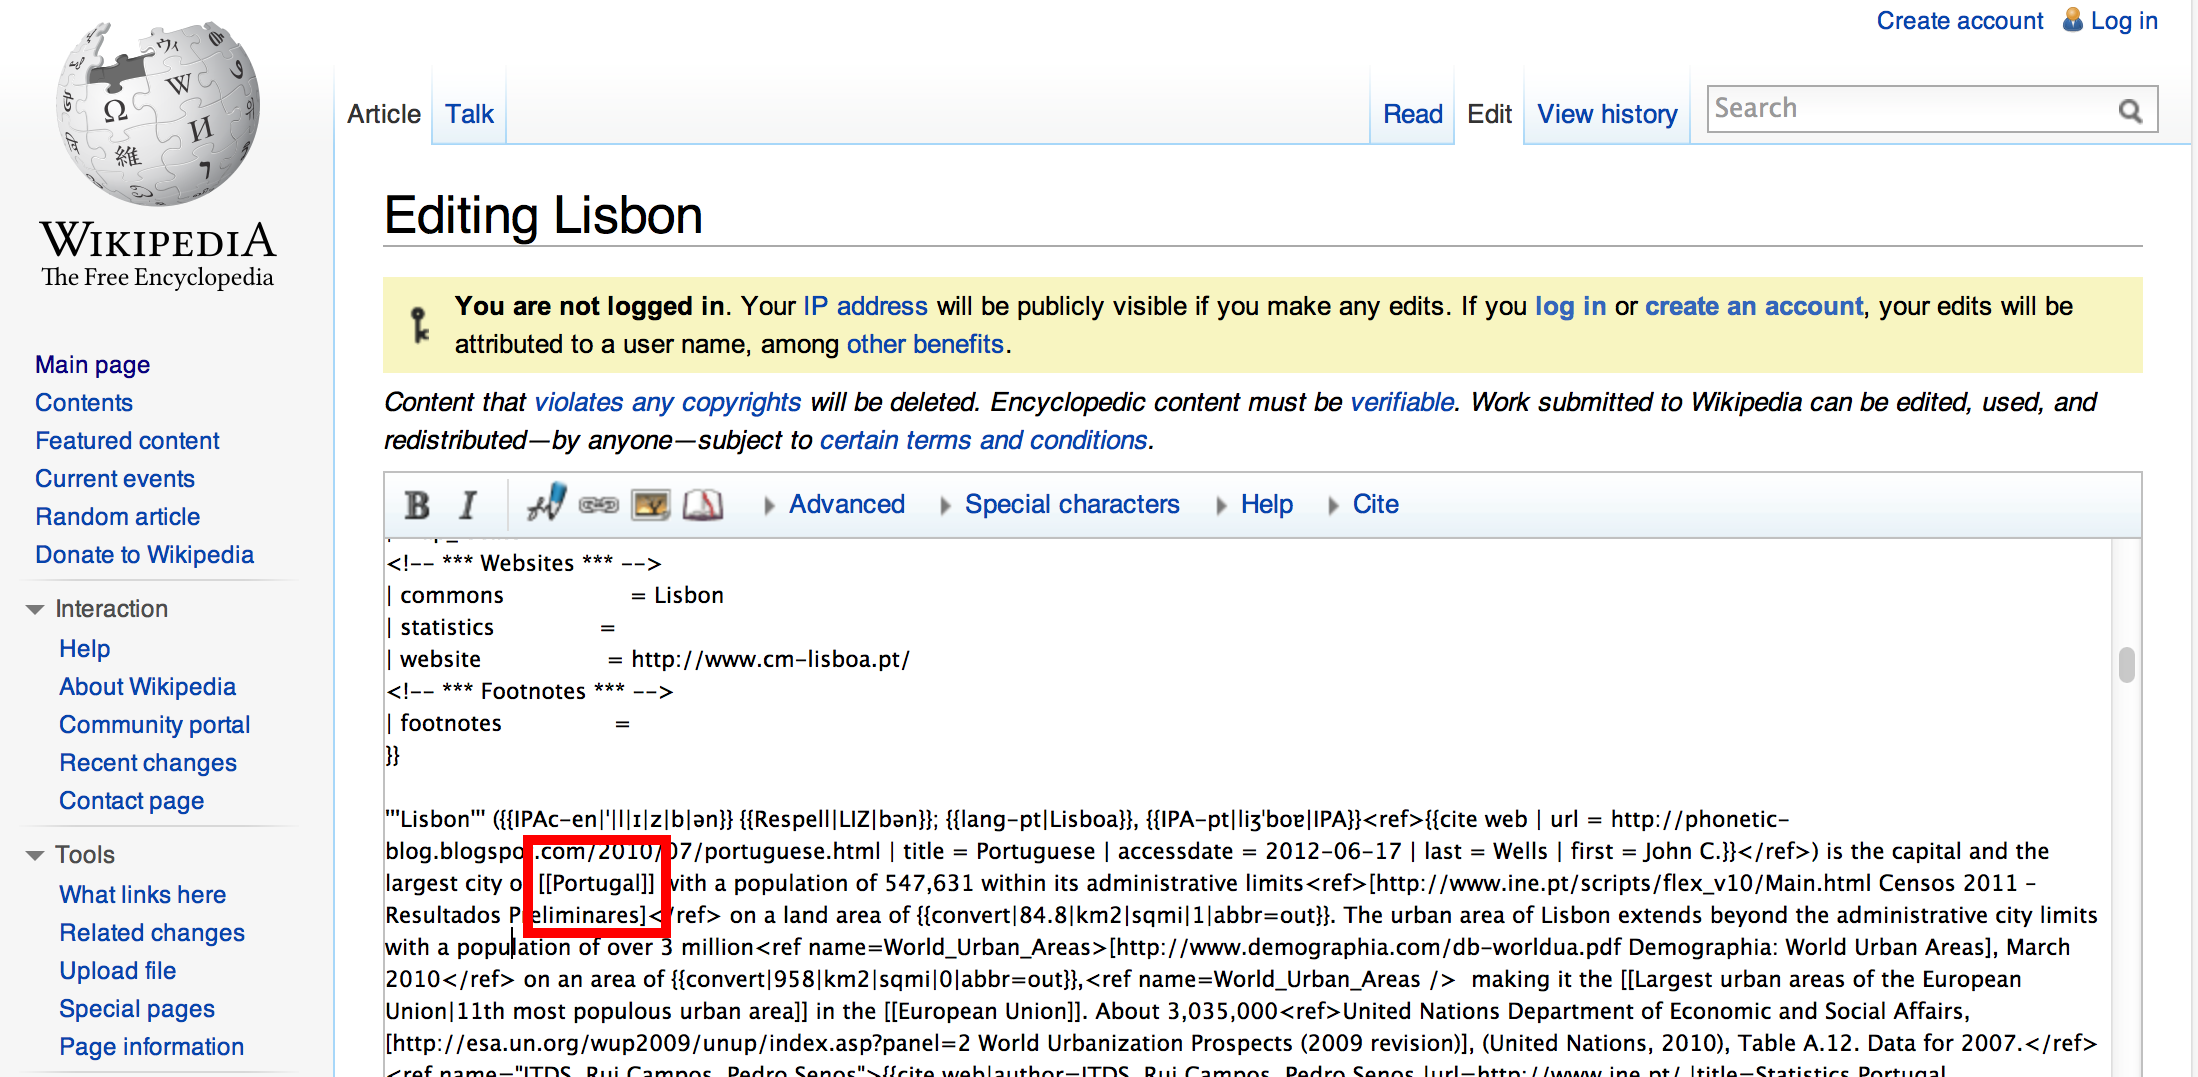
\includegraphics[scale=0.2]{pics/wikipedia_lisbon.png}
\end{figure}

Since everyone can edit any content, the submission of incorrect
content and vandalism can be expected. In
order to keep this under control, it is important that content is
versioned.
This way, when incorrect content or vandalism is discovered, the
version containing the problematic content can simply be removed. \\

\section{Some Wikipedia statistics}
To get a better idea about the needs of the Wikipedia platform in
terms of high-availability and scalability, let's take a look at some
statistics about Wikpedia.

\subsection{Presenting the statistics}
The Wikimedia foundation publishes statistics about all of their
products \cite{stats_wikimedia}. The general overview of Wikipedia
statistics \cite{stats_wikipedia} shows that the English Wikpedia is
the largest instance of all Wikipedia. Looking at the statistics for
this instance will be relevant to make assumptions in terms of
high-availability and scalability.
A summary of statistics is available for every Wikipedia instance.
We'll walk through the statistics summary of the English Wikipedia
instance, note that the presented charts are copies of the Wikipedia
statistics website \cite{stats_wikipedia}, downloaded January $7^{th}$
2014.\\
The total number of articles seems to increase linearly (see \cref{wikipedia_nr_articles_over_time}).
\begin{figure}[h!]
  \caption{Total number of English wikipedia articles over time}
  \label{wikipedia_nr_articles_over_time}
  \centering
    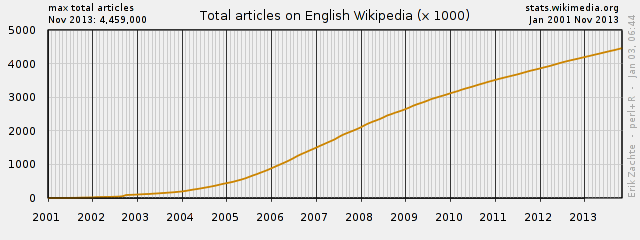
\includegraphics[scale=0.5]{pics/wikipedia_nr_articles_over_time.png}
\end{figure}
The amount of new articles per month seems to stay pretty much the
same over the last 5 years, however, there were some peaks earlier in
the history of Wikipedia (see \cref{wikipedia_nr_articles_over_time}).
\begin{figure}[h!]
  \caption{Number of new articles per month on the English Wikipedia}
  \label{wikipedia_new_articles_per_month}
  \centering
    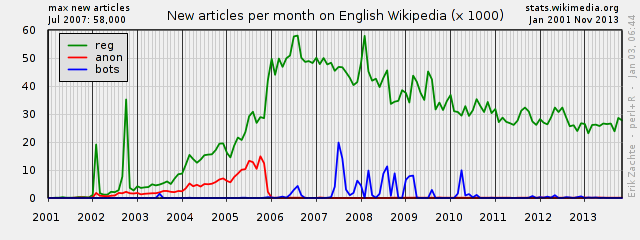
\includegraphics[scale=0.5]{pics/wikipedia_new_articles_per_month.png}
\end{figure}
The number of editors stays quite stable since the beginning of 2007
for frequent and very frequent editors. Since 2008, the number of
infrequent also has stabilised (see \cref{wikipedia_active_editors}). Between 2005 and 2007 there was a
steep growth (see \cref{wikipedia_active_editors}), but this growth was not
that spectacular in absolute numbers:
\begin{itemize}
\item 5+ edits: from $\approx 5000$ editors to $\approx 45000$ editors
\item 25+ edits: from $\approx 2000$ editors to $\approx 13000$ editors
\item 100+ edits: from $\approx 1000$ editors to $\approx 5000$ editors
\end{itemize}
\begin{figure}[h!]
  \caption{Active editors on the English Wikipedia}
  \label{wikipedia_active_editors}
  \centering
    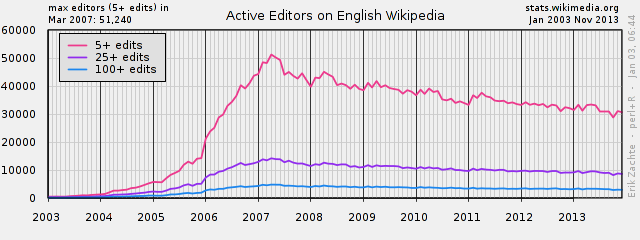
\includegraphics[scale=0.5]{pics/wikipedia_active_editors.png}
\end{figure}
The average number of edits per month is reported as $2,927,878$
edits.
The chart that summarises the number of page views per month shows 
a steady growth (see \cref{wikipedia_page_views}). The growth in absolute
numbers is significant:
\begin{itemize}
\item first quarter 2008: $\approx 4500$ million
\item first quarter 2013: $\approx 8400$ million
\end{itemize}
I was not able to find any statistics about page view count before
2008, but since Wikipedia only started in 2001, with only a
significant amount of articles since 2005 (see \cref{wikipedia_nr_articles_over_time}), we can assume that there
was a steep growth between 2005 and 2008.
\begin{figure}[h!]
  \caption{Number of page views per month on the English Wikipedia}
  \label{wikipedia_page_views}
  \centering
    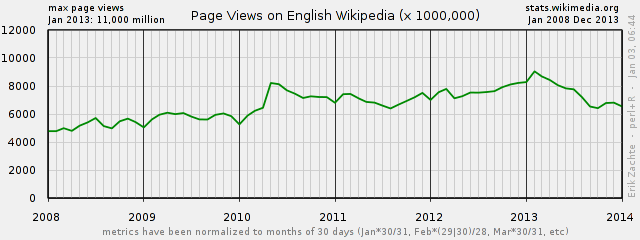
\includegraphics[scale=0.5]{pics/wikipedia_page_views.png}
\end{figure}
There were statistics about the growth of the Wikipedia database
\cite{wikipedia_database_growth}, but these statistics seem to be
discontinued. As to be expected, this database keeps growing linearly,
and there is no reason to assume this would change.
The actual articles do not take that much space: the XML dump of the
current database is only $\approx 44 GB$ \cite{wikipedia_size}. 
On the other hand, the database with all
revisions included is much bigger: \cite{wikipedia_size} reports it to be several
TBs after decompression (in 2010 this was $\approx 5TB$ \cite{wikipedia_full_size}).

\subsection{Interpretation of the statistics}
There is a significant different between the number of edits and the
number of views (per month).
The difference appears to be a factor $>1000$ over the last 6 years.
We can also see that the number of users (viewers) keeps growing
steadily (linearly) once the instance gained some popularity. 
From the moment an instance is started up until the moment an
instance gained popularity, a steep growth takes place; adding
millions of users (viewers) to the system over a period of a few
months/years.\\
The following high-availability and scalability requirements we need to meet:
\begin{itemize}
\item the possibility to handle a large number of
  simultaneous viewers: from the statistics we can expect $\approx 2500$
  requests per second
\item the possibility to easily scale in the number of viewers
\item the possibility to handle a moderate amount of editors: from the
  statistics we can expect $\approx 2.5$ requests per second
\item the content should be properly backup-ed and stored in a
  redundant way, since the content will grow incrementally the storage
  solution should allow to grow with it
\end{itemize}

\section{An attempt to setup an architecture}
Since there is clearly a difference in requirements between viewing content and
editing content, I think it would make sense to separate this
functionality.

\subsection{A few thoughts on storing the content with all revision
  information}
Wikimedia currently stores the Wikipedia data in databases. However,
it occurred to me that the data consists out of wikitext sections
(representing the articles) that have a history. So we could also
store this as a set of text files kept under revision control.
This would mean that we can store all articles and their history on a
plain file system.
Since we are interested at the history of one file at a time, using 
revision control such as git is overkill. A more efficient
approach would be to keep a directory with the name of the page and in
this directory store a set of patch files that represents the history of the
page.
For this to work, we would need to write a considerable amount of code, so for the
sake of this demonstration I will use git.
We expect our content to be $>$6TB (a reasonable assumption based on
the fact that it was $\approx 5TB$ in 2010). Currently there is raw
storage hardware available that supports up to 10TB
(\cite{hp_10TB_storage} for example), which should be
sufficient for at least 5 years of scalability.
Note that we could also opt for a ceph cluster \cref{ceph}, with a
practically unlimited scalability, however, for the current state of
affairs this might be overkill.
Several hardware solutions exist to setup this data storage in a
redundant way and make sure it is properly backup-ed. However it is
also necessary to make explicit incremental backups (since
we're storing the different revisions of our articles, this could be
done by only collecting the most recent revisions), these backups
should also be stored in a datacenter at another physical location.
The content storage server could than be implemented by a cluster of
redundant nodes with a unified interface, so that all other servers
can talk to this cluster as if it is only one machine.

\subsection{HTTP server for editors}
Since we only expect $\approx 2.5$ edits per second, this could be
handled by one machine that hosts a web application that allows
editing pages and communicates with the content storage server \footnote{To get
revisions and submit changes to content}.
If one server would no longer be sufficient to handle the load, an
additional web server could be used to setup an editor cluster, behind
a HAProxy proxy.

\subsection{HTTP server for viewers}
The current implementation of Wikipedia serves the content to viewers
using the MediaWiki software, which is PHP software that has to render
the pages on the server side before it can serve them to the user.
We no longer store the content in a a database, but as separate file, so
we might skip this rendering phase, and serve the files directly
\footnote{Seperating dynamic and static content is an optimization
  technique that is also advised by W. Tarreau of HAProxy \cite{haproxy:2013}}. 
Since we expect $>$2500 requests per second, we still need a cluster of
HTTP servers to handle this load. We can do that by using HAProxy as a 
front-end for our HTTP server cluster, this way, we can also easily add
extra HTTP servers to accommodate an increase in requests.
However, as mentioned before, our content is stored in wikitext
format, we cannot serve this directly to our viewers, since their
browser expects HTML. We can however pre-render the wikitext files (as
soon an edit was done on one of the files) and store the results of
this pre-rendering (an HTML file) directly on the HTTP servers that
are about to serve the content to our viewers \footnote{It is a
  realistic to want to keep a copy of the HTML file on each HTTP server,
since we know the dataset only containing the current version of
the files only takes $\approx 44GB$ (in XML format, we can assume the
HTML exports of the pages will be of similar size)}.

\section{Testing this architecture}
To test this architecture, we'll setup the following experiment:
\begin{itemize}
\item a content storage server 
\item a cluster of HTTP servers that can serve HTML files rendered from
the wiktext files on the content storage server, I will use my
existing HAProxy cluster for this (see \cref{ha_proxy_experiment})
\end{itemize}

\subsection{The content storage server}
I created a new virtual machine named 'content' by clone my base
Ubuntu virtual machine.
To install git (what I will use to handle the revision control):
\begin{lstlisting}[language=bash]
sudo apt-get install git
\end{lstlisting}
Let's git know who we are:
\begin{lstlisting}[language=bash]
git config --global user.name "plibin"
git config --global user.email "pieter.libin@vub.ac.be"
\end{lstlisting}

Now we can setup the server git repository \cite{git_setup_server}
\footnote{Make sure to add this group and the $--shared=group$ option,
if not you WILL have problems, unfortunately this is not mentioned in
the the git documentation}: 
\begin{lstlisting}[language=bash]
cd /var/
sudo addgroup gituser
sudo mkdir wiki-pages.git
sudo chown -R plibin:gituser wiki-pages.git
cd wiki-pages.git
git --bar init --shared=group
\end{lstlisting}
To properly initialise the server repository, we need to push
something to it (still on 'content') \cite{git_setup_server}:
\begin{lstlisting}[language=bash]
cd /home/plibin
mkdir wiki-pages
cd wiki-pages
git init
echo "Wikipedia experiment" > Readme
git add Readme
git commit -m 'initial commit'
git remote add origin /var/wiki-pages.git
git push origin master
\end{lstlisting}

We need to make it possible for  'content' to contact 'node1' and
'node2' whenever a new (git) push is received by 'content'. The
easiest way to do this is by letting 'content' executing a remote command on
the nodes via ssh.\\
In order to do this we need to configure the nodes so that we do not
need to provide a password when logging in with ssh. 
We can do this by executing the following commands (on 'content')
\footnote{I added 'node1' and 'node2' to 'content's /etc/hosts file}:
\begin{lstlisting}[language=bash]
ssh-keygen
ssh-copy-id node1
ssh-copy-id node2
\end{lstlisting}

Now we need to add a hook to our git repository (on 'content) that
executes an update-script on our nodes ('node1' and 'node2')
\cite{git_hooks}.
We need to add a 'post-receive' hook, such a hook is triggered
whenever the git repository receives a push.
To add such a hook:
\begin{lstlisting}[language=bash]
cd /var/wiki-pages.git
echo "ssh plibin@node1 /home/plibin/update-wiki-pages.sh" 
  >> ./hooks/post-receive
echo "ssh plibin@node2 /home/plibin/update-wiki-pages.sh" 
  >> ./hooks/post-receive
chmod +x ./hooks/post-receive
\end{lstlisting}

\subsection{The HTTP nodes}
Now we need to provide an update-wiki-pages.sh script on the 2 nodes,
this script will:
\begin{itemize}
\item do a git pull to get the latest content from the storage server
'content'
\item convert all files (that are in wikitext form: more specifically
  in the creole dialect \cite{creole_dialect}) to HTML; for this I use
  the txt2tags program \footnote{Updating all files is not efficient;
    in a production environment we would only update  the files that actually changed}
\end{itemize}

The code for this script:
 \begin{lstlisting}[language=bash]
src/wikipedia/update-wiki-pages.sh
\end{lstlisting}
This script calls another simple script that converts a creole file to
an HTML file:
 \begin{lstlisting}[language=bash]
src/wikipedia/creole2html.sh
\end{lstlisting}

We need to install txt2tags to convert the Creole files to HTML and git (this
command should be executed on 'node1' and 'node2'):
\begin{lstlisting}[language=bash]
sudo apt-get install txt2tags
sudo apt-get install git
\end{lstlisting}

To make sure that this script can do its job, we need to clone the git
repository from the 'content' server on both nodes ('node1' and 'node2'):
 \begin{lstlisting}[language=bash]
cd ~
git clone content:/var/wiki-pages
\end{lstlisting}
We now also need to be able to contact 'content' over ssh without using
a password (these commands should be executed on 'node1' and 'node2'):
\begin{lstlisting}[language=bash]
ssh-keygen
ssh-copy-id content
\end{lstlisting}

To configure the web server, we simply need to make a link to our
wiki-pages git repository in /var/www \footnote{Simply making a
  symbolic links allows the users to also see the .crl files, which is
  not our intention, this can be fixed by configuring Apache to only
  show HTML files.}:
\begin{lstlisting}[language=bash]
cd /var/www/
sudo ln -s ~/wiki-pages/ wiki
\end{lstlisting}

\subsection{Testing the setup}
After adding a ``Portugal''-page and ``Lisbon''-page that references
the Portugal page in Creole format to the content storage server, the
wiki seems to work fine (as can be seen in \cref{fig:wikipedia_clone_1}).

\begin{figure}[h!]
  \caption{Accessing our wiki via HAProxy (haproxy server has
    IP-address 192.168.15.10)}
  \label{fig:wikipedia_clone_1}
  \centering
    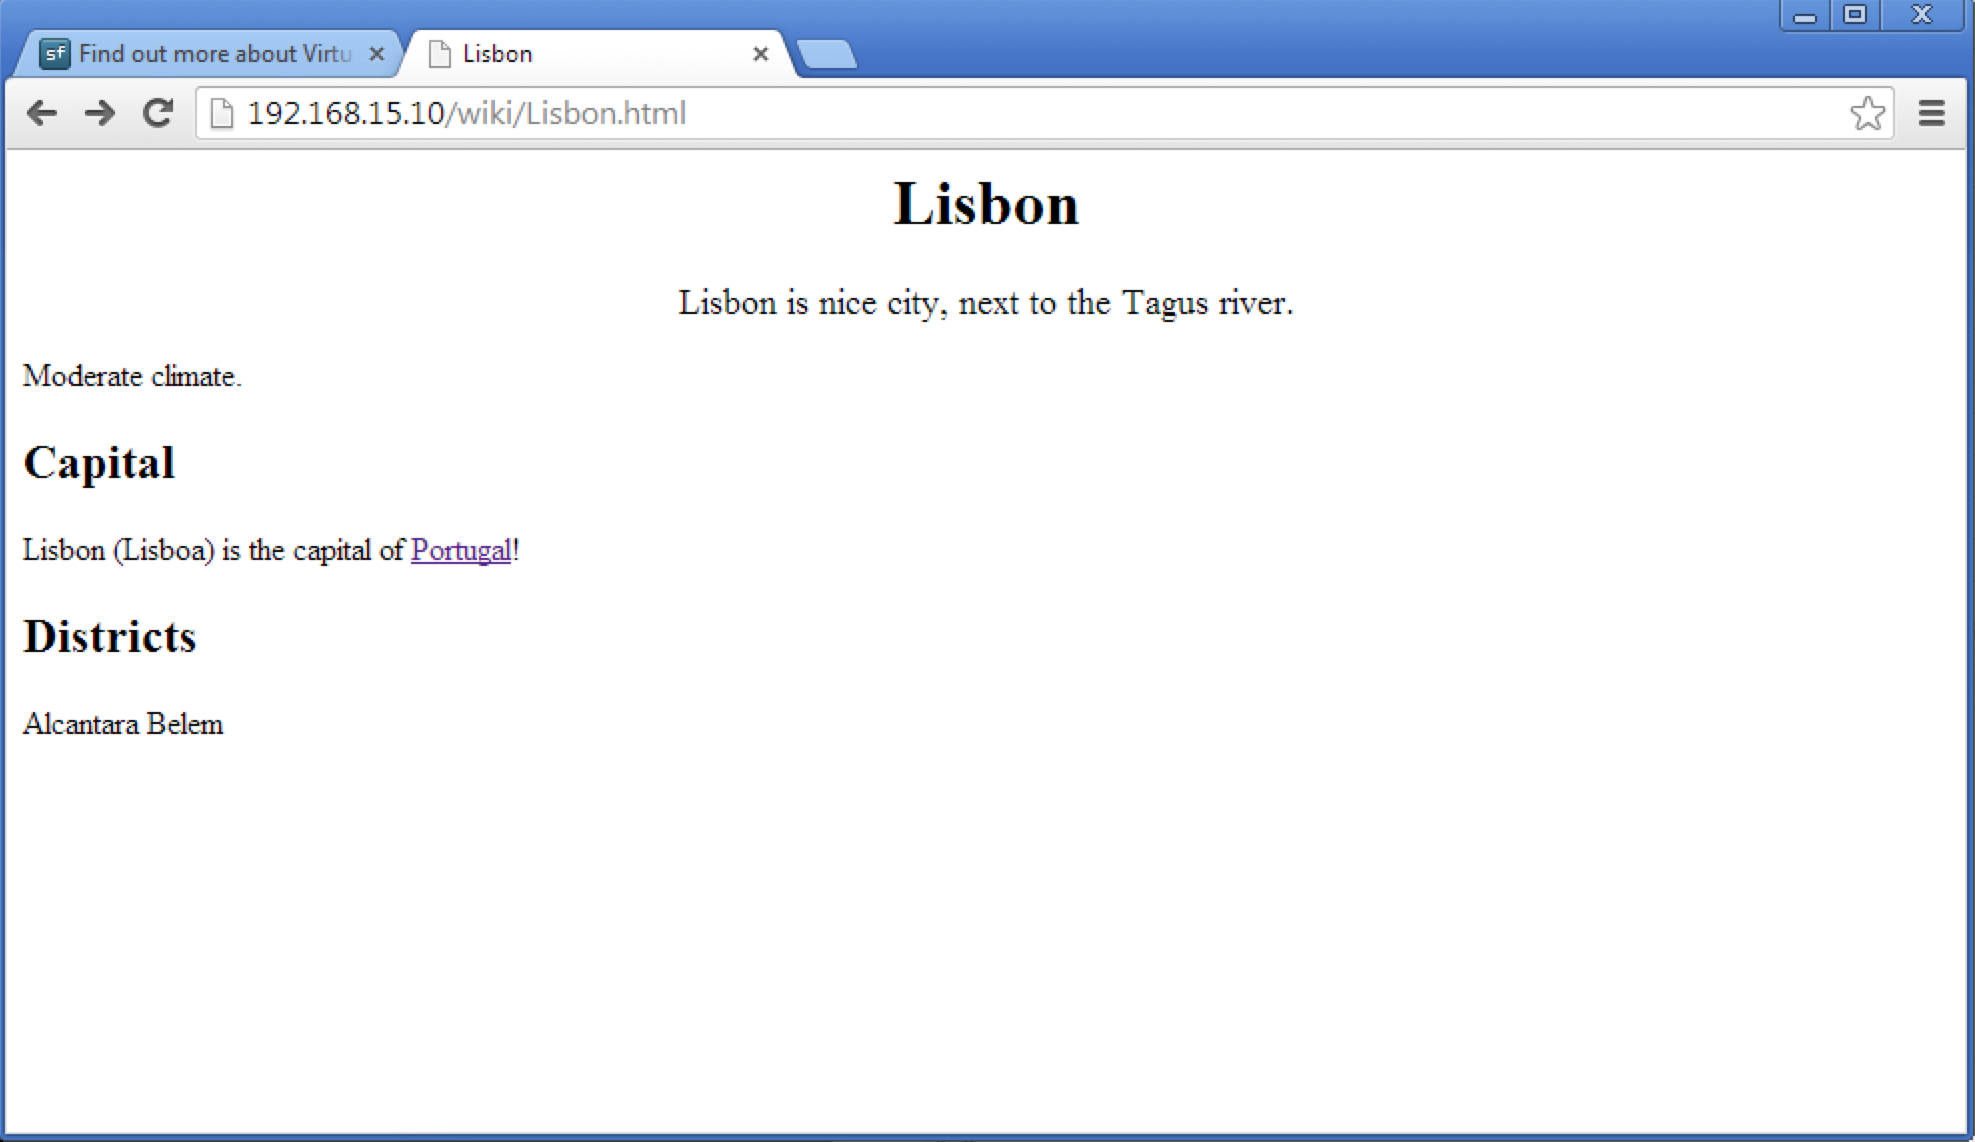
\includegraphics[scale=0.2]{pics/wikipedia_clone_1.png}
\end{figure}

I recorded a video where I add another page about ``Faial'', which is
an island in the Portuguese Azorean archipelago:\\
https://www.youtube.com/watch?v=zk-Ny046kuw
\\
I recorded another short video where I add a link to Portugal on the
Faial page:
https://www.youtube.com/watch?v=T-\_baLRBBfE


\subsection{Conclusion and remarks}
In my opinion, my architecture should be able to handle a website such as
Wikipedia (although some additional developments would be
necessary). 
\subsubsection{Performance}
When looking at some benchmarks
(\cite{web_server_benchmarks}); if we expect 2500 requests per second,
we would only need a couple of servers to handle this. Other web
servers such as lighthttpd and nginx seem to do event better with
static content. \\
However, to make any serious claims about the amount of servers that
would be needed, we need to perform a large-scale performance test,
which is out of the scope of this experiment.
\subsubsection{Simplifications}
I had to make some simplifications in my setup; the most important one
being that there is no support for any dynamic content in the pages. This
is however necessary for certain parts of a page (e.g.: to
calculate the age of a person), however, most of these computations
can also be done in JavaScript. If there would be computations that
cannot be done in JavaScript, it would still be possible to let
JavaScript invoke a REST service to do this computation.   

\chapter{Conclusion} % Major section
\section{State of the art}
There exist tons of open-source softwares developed for the GNU/Linux 
operating system that allow to build scalable and available systems.
The quality of this software varies, but in general, most of this
software is in good shape. \\
I executed several experiments, and I did not run into a lot of
bugs. However, for quite some projects, the documentation was not
really up to date. Because of this, I often had to lookup various
documents and tutorial.\\

\section{What did I learn}
I really enjoyed experimenting with these different technologies a lot. I
learned a lot how these technologies work (architecture-wise) and how
they can be installed and used.\\
I covered several aspects of scalable and available system design and
development: 
\begin{itemize}
\item I studied existing technologies and their architecture
\item I installed and configured existing technologies in a simulated
  environment (virtualised cluster)
\item I wrote specific softwares to explore the development aspect of
  this domain
\item I thought through an architecture and system design for a
  real-world scenario
\end{itemize}
Working through these different aspects thought me a lot about the
domain. 

\section{What does this project contribute}
First of all, I learned a huge amount by executing this project, so it
was really valuable for my personal and professional development.\\
I think this project gives an overview of a lot of different aspects
that are relevant in the domain of scalable and available
clusters. The project provides a theoretical foundation, explores
some of the solutions and executes real-world experiments.\\
 I tried to
thoroughly document the different steps of the experiment, to ensure
the reader can reproduce all experiments \footnote{I thought it was
  important to be thorough in this documentation, since very often, I
  had to consult many different tutorials. I hope this document can
  act as a starting point for executing similar experiments,
  alleviating the need to browse through tons of different
  documentation files.}. When documenting these steps
I often based my work on tutorials and documentation that I found
online or in books, I always tried to accurately reference to these
documents to avoid any plagiarism.

%----------------------------------------------------------------------------------------
%	BIBLIOGRAPHY
%----------------------------------------------------------------------------------------



\bibliography{mybib}{}
\bibliographystyle{ieeetr}

%----------------------------------------------------------------------------------------

\end{document}
